\documentclass[aspectratio=169,10pt]{beamer}

% ── Theme & Colors ──────────────────────────────────────────
\usetheme{metropolis}
\usepackage{appendixnumberbeamer}
\usepackage{booktabs}
\usepackage{amsmath,amssymb}
\usepackage{tikz}
\usetikzlibrary{arrows.meta,positioning,calc,decorations.pathreplacing,shapes.geometric}
\usepackage{pgfplots}
\pgfplotsset{compat=1.18}
\usepackage{xcolor}
\usepackage{graphicx}
\usepackage{multicol}

% Columbia-inspired palette
\definecolor{columbia}{RGB}{29,79,145}
\definecolor{columbialight}{RGB}{117,170,219}
\definecolor{columbiaaccent}{RGB}{210,73,42}
\definecolor{columbiagray}{RGB}{117,117,117}
\definecolor{softbg}{RGB}{245,245,250}
\definecolor{warnbg}{RGB}{255,240,230}

\setbeamercolor{frametitle}{bg=columbia,fg=white}
\setbeamercolor{progress bar}{fg=columbiaaccent}
\setbeamercolor{alerted text}{fg=columbiaaccent}
\setbeamercolor{block title}{bg=columbia,fg=white}
\setbeamercolor{block body}{bg=softbg}

\setbeamerfont{title}{size=\Large,series=\bfseries}
\setbeamerfont{frametitle}{size=\large,series=\bfseries}

% ── Metadata ────────────────────────────────────────────────
\title{Health Data Modalities I:\\EHR \& Claims Data}
\subtitle{BINF 4002 --- Machine Learning for Health \quad$\cdot$\quad Lecture 17}
\author{Matthew McDermott}
\date{March 24, 2026}
\institute{Department of Biomedical Informatics\\Columbia University}

% ── Document ────────────────────────────────────────────────
\begin{document}

% ============================================================
% TITLE
% ============================================================
\maketitle

% ============================================================
% SECTION 0: FRAMING
% ============================================================


% ============================================================
% SECTION 0: FRAMING
% ============================================================


\section{From ML Fundamentals to Health AI}



\begin{frame}{The Second Half of the Course}
\begin{columns}[T]
\begin{column}{0.48\textwidth}
\textbf{Where we've been:}
\begin{itemize}
    \item Math foundations (LA, probability, optimization)
    \item ML theory (training, evaluation, model types, loss types, algorithms)
    \item Foundation models \& LLMs
\end{itemize}
\end{column}
\begin{column}{0.48\textwidth}
\textbf{Where we're going:}
\begin{itemize}
    \item \alert{Health data modalities} (Lectures 17--20)
    \item Health-specific models \& methods (Lectures 21--25)
    \item Deployment challenges (Lectures 26--27)
\end{itemize}
\end{column}
\end{columns}

\vspace{1em}
\textbf{The pattern for each modality:}
\begin{enumerate}
    \item Map it to the ML data taxonomy from our data types discussions
    \item Identify where the mapping \emph{breaks}
    \item Understand the implications for modeling
\end{enumerate}
\end{frame}




\begin{frame}{Today's Plan}
\begin{enumerate}
    \item \textbf{A statistical trap} --- a puzzle to keep in mind \hfill\textcolor{columbiagray}{\scriptsize 5 min}
    \item \textbf{EHR \& claims data} --- what they are, what's in them \hfill\textcolor{columbiagray}{\scriptsize 10--30 min}
    \item \textbf{The complexity of health data} --- a roadmap \hfill\textcolor{columbiagray}{\scriptsize 30--35 min}
    \item \textbf{Cohort selection examples} --- where the pitfalls live \hfill\textcolor{columbiagray}{\scriptsize 35--60 min}
    \item \textbf{Returning to the trap} --- Berkson's Paradox in practice \hfill\textcolor{columbiagray}{\scriptsize 60--68 min}
    \item \textbf{Standards \& takeaways} \hfill\textcolor{columbiagray}{\scriptsize 68--75 min}
\end{enumerate}

\vspace{0.3em}
\textbf{Reminder:} Midterm is due today.
\end{frame}

\section{A Statistical Trap}

\begin{frame}{Do You See a Pattern?}
\vspace{-0.5em}
\begin{center}
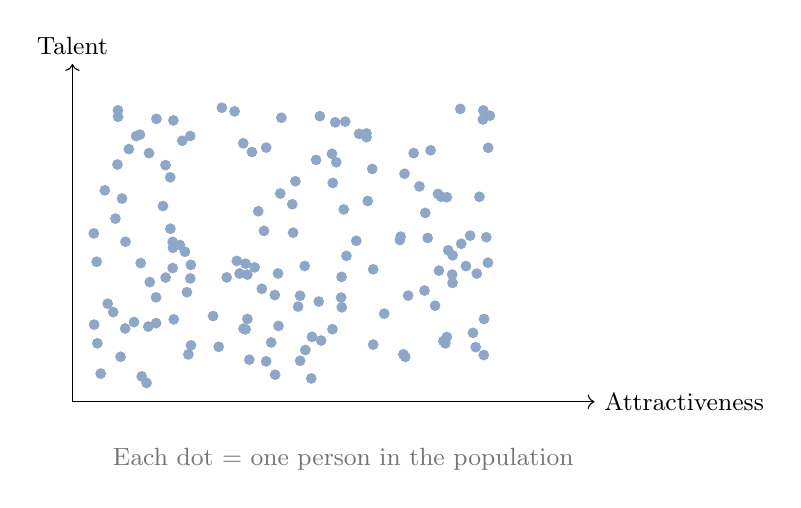
\begin{tikzpicture}[scale=0.78]
    \draw[->] (0,0) -- (8.5,0) node[right, font=\small] {Attractiveness};
    \draw[->] (0,0) -- (0,5.5) node[above, font=\small] {Talent};

    \pgfmathsetseed{42}
    \foreach \i in {1,...,150} {
        \pgfmathsetmacro{\x}{0.3 + 6.5*rnd}
        \pgfmathsetmacro{\y}{0.3 + 4.5*rnd}
        \fill[columbia!50] (\x, \y) circle (2.5pt);
    }
    \node[font=\small, columbiagray, anchor=north west] at (0.5, -0.6) {Each dot = one person in the population};
\end{tikzpicture}
\end{center}

\pause
\centering No pattern. Attractiveness and talent are \textbf{independent} in the general population.
\end{frame}

\begin{frame}{What If You Can Only Observe Celebrities?}
\begin{center}
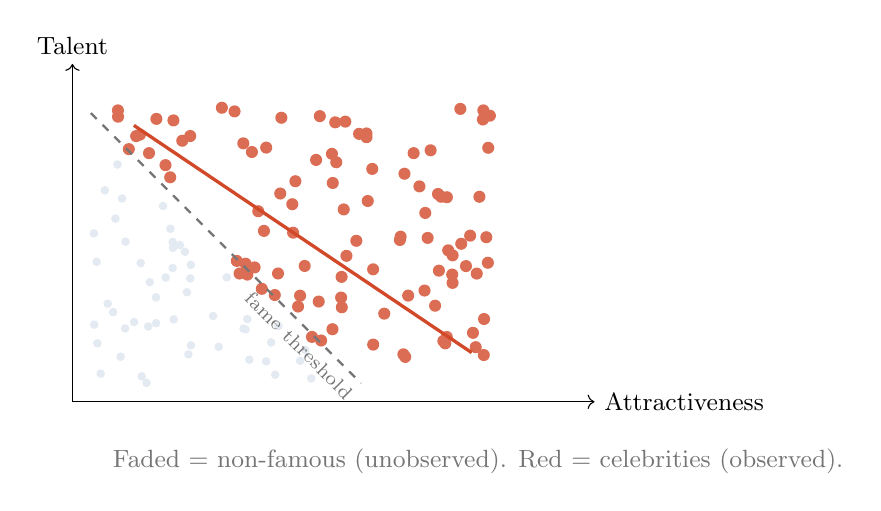
\begin{tikzpicture}[scale=0.78]
    \draw[->] (0,0) -- (8.5,0) node[right, font=\small] {Attractiveness};
    \draw[->] (0,0) -- (0,5.5) node[above, font=\small] {Talent};

    \pgfmathsetseed{42}
    \foreach \i in {1,...,150} {
        \pgfmathsetmacro{\x}{0.3 + 6.5*rnd}
        \pgfmathsetmacro{\y}{0.3 + 4.5*rnd}
        \pgfmathsetmacro{\total}{\x + \y}
        \ifdim \total pt > 4.7pt
            \fill[columbiaaccent!80] (\x, \y) circle (2.8pt);
        \else
            \fill[columbia!12] (\x, \y) circle (2pt);
        \fi
    }
    \draw[dashed, columbiagray, thick] (0.3, 4.7) -- (4.7, 0.3)
        node[pos=0.6, below right, font=\scriptsize\color{columbiagray}, rotate=-45] {fame threshold};
    \draw[very thick, columbiaaccent] (1.0, 4.5) -- (6.5, 0.8);
    \node[font=\small, columbiagray, anchor=north west] at (0.5, -0.6) {Faded = non-famous (unobserved). Red = celebrities (observed).};
\end{tikzpicture}
\end{center}
\pause
\vspace{-0.3em}
Among celebrities, attractive ones \emph{seem} less talented. \textbf{But this is an illusion} --- you're only seeing the top-right slice of an uncorrelated cloud.
\end{frame}

\begin{frame}{This Has a Name: Berkson's Paradox (1946)}
\begin{columns}[T]
\begin{column}{0.45\textwidth}
\begin{alertblock}{The Mechanism}
When you \textbf{condition on a collider} --- a variable caused by two others --- you create a \textbf{spurious correlation} between those causes.
\end{alertblock}

\vspace{0.5em}
\textbf{Causal diagram:}
\begin{center}
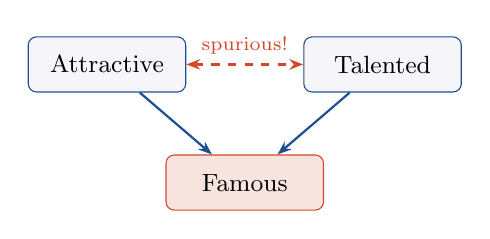
\begin{tikzpicture}[
    node distance=1.2cm,
    var/.style={draw=columbia, fill=softbg, rounded corners=3pt,
                minimum width=2cm, minimum height=0.7cm, align=center, font=\small},
    arr/.style={-{Stealth[length=5pt]}, thick, columbia}
]
\node[var] (A) at (0, 0) {Attractive};
\node[var] (B) at (3.5, 0) {Talented};
\node[var, draw=columbiaaccent, fill=columbiaaccent!15] (C) at (1.75, -1.5) {Famous};
\draw[arr] (A) -- (C);
\draw[arr] (B) -- (C);
\draw[thick, columbiaaccent, dashed, {Stealth[length=5pt]}-{Stealth[length=5pt]}]
    (A) -- node[above, font=\scriptsize\color{columbiaaccent}] {spurious!} (B);
\end{tikzpicture}
\end{center}
\end{column}
\begin{column}{0.50\textwidth}
\pause
\textbf{The pattern:}
\begin{enumerate}
    \item Two variables (A, B) are independent
    \item Both cause a third variable (C)
    \item You only observe data \emph{where C occurred}
    \item A and B now appear correlated
\end{enumerate}
\vspace{0.5em}
\pause
\textbf{Other examples:}
\begin{itemize}
    \item Restaurants: good food \emph{or} good ambiance (you don't eat at places with neither)
    \item Universities: high GPA \emph{or} high SAT (you only see admitted students)
\end{itemize}
\end{column}
\end{columns}
\end{frame}

\section{Refresher: Data Types You Already Know}

\begin{frame}{The ML Data Zoo}
From the labs, you've worked with five broad data modalities:

\vspace{0.4em}
\begin{center}
\begin{tabular}{lll}
\toprule
\textbf{Modality} & \textbf{Structure} & \textbf{Health Example} \\
\midrule
Tabular & Fixed-length feature vector $\mathbf{x} \in \mathbb{R}^d$ & Breast cancer features \\
Graph & Nodes + edges $(V, E)$ & Protein interaction nets \\
Text & Token sequence $(w_1, \ldots, w_T)$ & Clinical notes (later!) \\
Image & Pixel grid $\mathbb{R}^{H \times W \times C}$ & Skin lesion images \\
Time series & Regular grid $(x_1, \ldots, x_T)$ & ECG waveforms \\
\bottomrule
\end{tabular}
\end{center}

\end{frame}

\begin{frame}{What Makes EHR Data Different?}
\begin{columns}[T]
\begin{column}{0.48\textwidth}
\textbf{Desired ML data:}
\begin{itemize}
    \item Collected \emph{for} analysis
    \item Fixed feature set across samples
    \item Observations at regular/designed intervals
    \item Samples are independent
    \item Missing data is ``incidental''
\end{itemize}
\end{column}
\begin{column}{0.48\textwidth}
\textbf{EHR data:}
\begin{itemize}
    \item<2-> \alert{Byproduct} of clinical care
    \item<3-> Variable features per patient
    \item<4-> Events at \emph{irregular}, \emph{informative} times
    \item<5-> Patients share providers, wards, policies
    \item<6-> Missing data is \emph{the norm} and \emph{informative}
\end{itemize}
\end{column}
\end{columns}


\vspace{0.5em}
\uncover<7->{
Think of it this way: a tabular dataset is like a \textbf{spreadsheet someone designed}. An EHR is like \textbf{receipts, sticky notes, and lab printouts from 15 departments} that you're now trying to analyze.
}
\end{frame}

% ============================================================
% SECTION 2: WHAT IS AN EHR?
% ============================================================




\section{What Is an Electronic Health Record?}

\begin{frame}{The EHR Is Not a Dataset}
\begin{alertblock}{Key Insight}
EHR data is a \textbf{byproduct of clinical care}, not a designed measurement instrument.
\end{alertblock}

\vspace{0.5em}
\begin{columns}[T]
\begin{column}{0.55\textwidth}
\textbf{What generates EHR data:}
\begin{itemize}[<+->]
    \item Clinician documentation (notes, orders)
    \item Lab systems (results, reference ranges)
    \item Billing / coding (ICD, CPT, LOINC)
    \item Nursing flowsheets (vitals, I/O)
    \item Pharmacy (medication orders, dispensing)
\end{itemize}
\end{column}
\begin{column}{0.42\textwidth}
\textbf{Implications:}
\begin{itemize}[<+->]
    \item Data reflects \emph{what was done}, not everything that happened
    \item Absent data $\neq$ absent condition
    \item Coding reflects billing incentives, not just clinical reality
    \item Each hospital's EHR is a different ``dialect''
\end{itemize}
\end{column}
\end{columns}
\end{frame}


\begin{frame}{What Does an EHR Look Like?}
\begin{center}
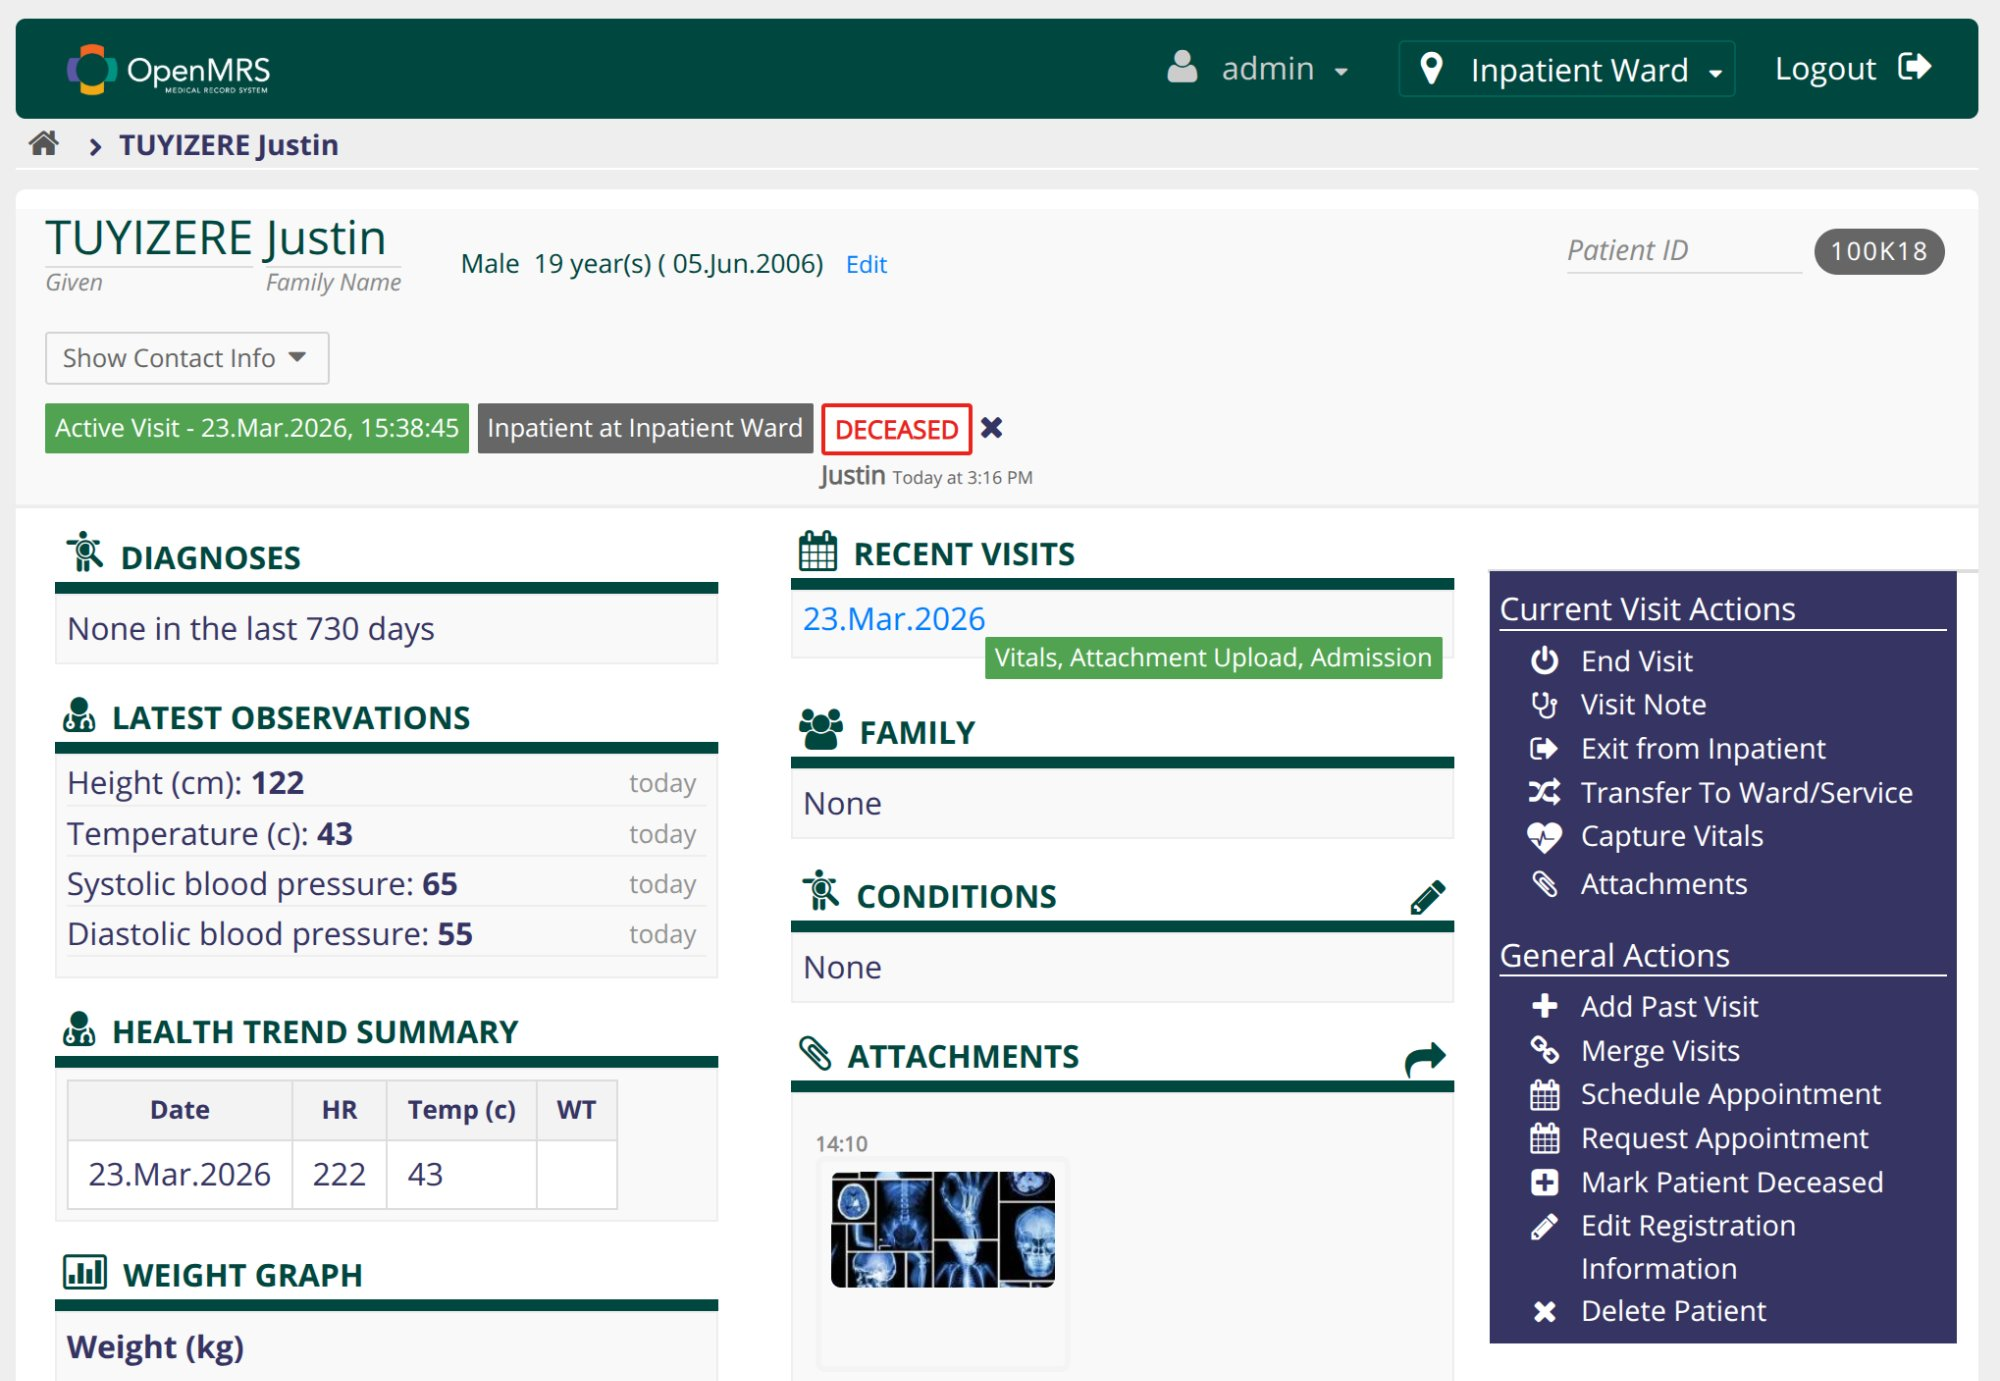
\includegraphics[width=0.88\textwidth]{figures/openmrs_screenshot.png}
\end{center}

\vspace{-0.3em}
\scriptsize Screenshot from \textbf{OpenMRS} --- an open-source EHR used in 6,500+ facilities worldwide. Note the patient banner, diagnoses, vitals, visit history, and action menu. Try it yourself: \url{https://demo.openmrs.org/openmrs/}
\end{frame}


\begin{frame}{Anatomy of a Patient Record}
\begin{center}
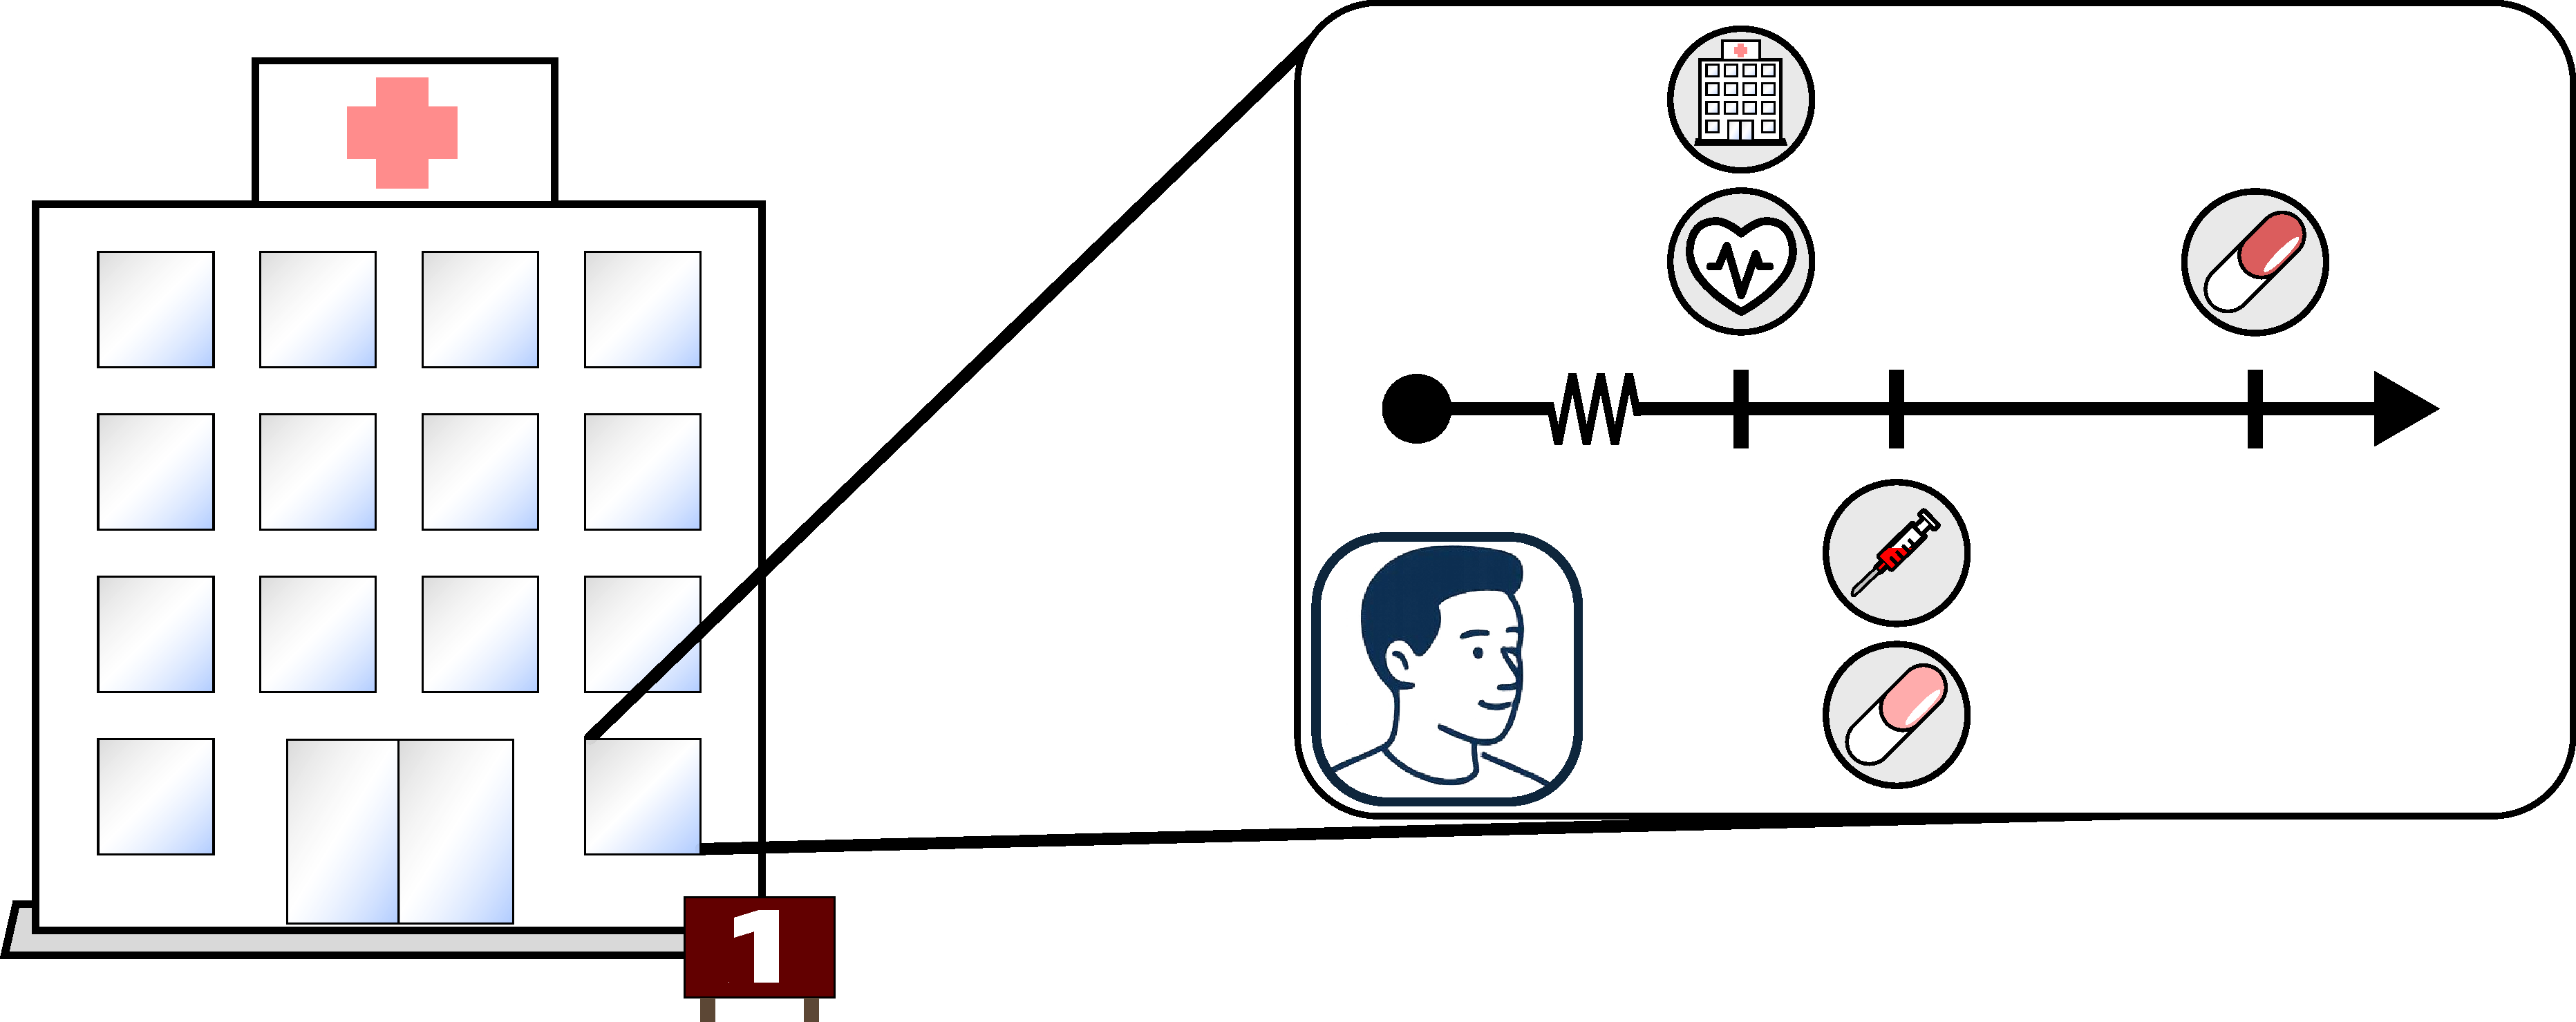
\includegraphics[width=0.65\textwidth]{figures/timeline.pdf}
\end{center}

\vspace{-0.3em}
\small
\begin{itemize}\setlength{\itemsep}{1pt}
    \item Events arrive at \textbf{irregular} times --- not a regular time series!
    \item Each event has a \textbf{code} (ICD, LOINC, RxNorm, \ldots) and optionally a \textbf{value}
    \item \textbf{Gaps carry information} --- why no data for 5 months?
\end{itemize}
\end{frame}


% ============================================================
% SECTION 3: WHAT IS CLAIMS DATA? (MOVED UP)
% ============================================================


\section{What Is Claims Data?}



\begin{frame}{What Are Claims Data?}
\begin{alertblock}{Definition}
\textbf{Claims data} are records generated when a healthcare provider submits a bill to an insurance payer. They document what services were provided and the diagnoses that justified them.
\end{alertblock}

\vspace{0.3em}
Same event-stream structure as EHR --- but with critical differences:

\vspace{0.2em}
\begin{center}
\scriptsize
\begin{tabular}{p{2.8cm}p{4.8cm}p{4.8cm}}
\toprule
\textbf{Dimension} & \textbf{EHR Data} & \textbf{Claims Data} \\
\midrule
\visible<2->{\textbf{Generating process}} & \visible<2->{Clinical care documentation} & \visible<2->{Insurance billing} \\
\visible<3->{\textbf{Temporal resolution}} & \visible<3->{Event-level (minutes)} & \visible<3->{Claim-level (days--weeks)} \\
\visible<4->{\textbf{Clinical depth}} & \visible<4->{Lab values, vitals, notes} & \visible<4->{Codes and costs only} \\
\visible<5->{\textbf{Population breadth}} & \visible<5->{Single institution} & \visible<5->{Entire payer network} \\
\visible<6->{\textbf{Completeness}} & \visible<6->{Within-system only} & \visible<6->{Across providers} \\
\bottomrule
\end{tabular}
\end{center}
\end{frame}

\begin{frame}{Types of Claims Data}
\begin{columns}[T]
\begin{column}{0.48\textwidth}
\textbf{Claim types (by form):}
\vspace{0.2em}

\scriptsize
\begin{tabular}{p{1.8cm}p{4cm}}
\toprule
\textbf{Type} & \textbf{Content} \\
\midrule
Professional (CMS-1500) & Physician/outpatient; DX + CPT codes \\
Institutional (UB-04) & Hospital; DRGs, revenue codes, LOS \\
Pharmacy (NCPDP) & NDC drug code, days supply, cost \\
\bottomrule
\end{tabular}
\end{column}
\begin{column}{0.48\textwidth}
\textbf{Payer types:}
\vspace{0.2em}

\scriptsize
\begin{tabular}{p{1.8cm}p{4cm}}
\toprule
\textbf{Payer} & \textbf{Key facts} \\
\midrule
Medicare & Elderly/$\geq$65; largest US claims DB \\
Medicaid & Low-income; varies by state \\
Commercial & Employed; MarketScan, Optum \\
VA & Veterans; capitation (not FFS) \\
\bottomrule
\end{tabular}
\end{column}
\end{columns}

\vspace{0.8em}
\textbf{Why this matters for ML:}
\begin{itemize}
    \item \textbf{FFS} (fee-for-service) pays per claim $\Rightarrow$ incentivizes volume and upcoding
    \item \textbf{Capitated} plans pay fixed amounts $\Rightarrow$ incentivizes under-documentation
    \item The \emph{same patient's} claims look different depending on their insurance type
\end{itemize}
\end{frame}


\begin{frame}{What Does a Claim Look Like?}
\begin{columns}[T]
\begin{column}{0.48\textwidth}
\begin{center}
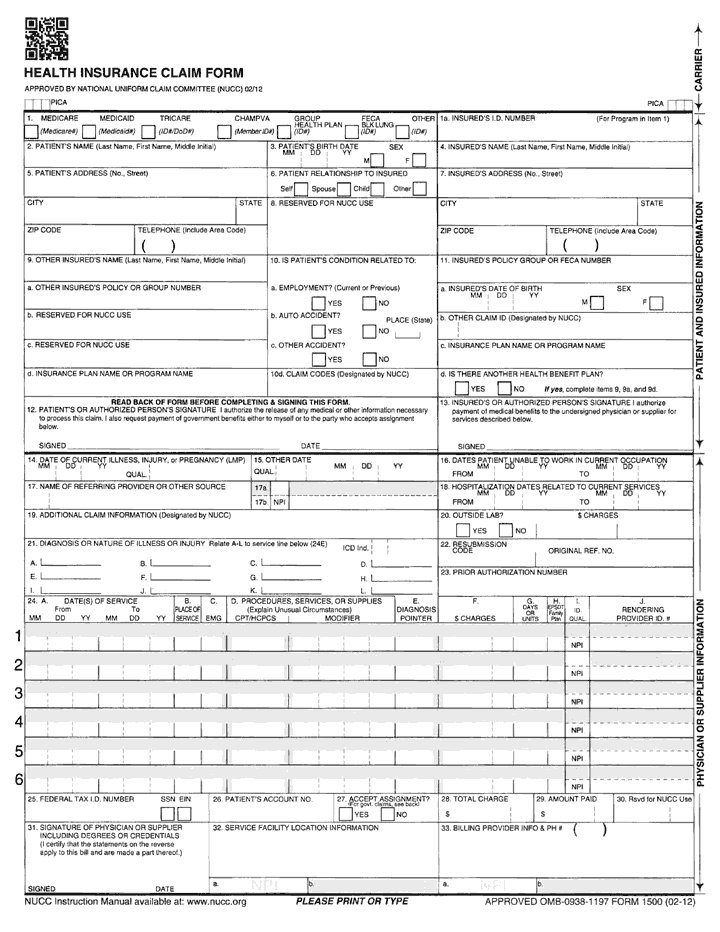
\includegraphics[width=\textwidth]{figures/cms1500_form.png}
\end{center}
\end{column}
\begin{column}{0.48\textwidth}
\small
\textbf{What's on a CMS-1500:}
\begin{itemize}\setlength{\itemsep}{1pt}
    \item Patient demographics
    \item \textbf{ICD-10 diagnosis codes} (Box 21)
    \item \textbf{CPT procedure codes} (Box 24)
    \item Place of service
    \item Charges, provider info
\end{itemize}

\vspace{0.3em}
\textbf{What's NOT on a CMS-1500:}
\begin{itemize}\setlength{\itemsep}{1pt}
    \item Lab values (just the order code)
    \item Vital signs
    \item Clinical notes
    \item Medication doses
    \item Anything not coded
\end{itemize}
\end{column}
\end{columns}
\end{frame}


% ============================================================
% SECTION 4: FEATURE DIMENSIONALITY
% ============================================================


\section{Comparing EHR \& Claims}




\begin{frame}{The Landscape of Health Data Features}
\begin{center}
\scriptsize
\begin{tabular}{lll}
\toprule
\textbf{Dimension} & \textbf{EHR} & \textbf{Claims} \\
\midrule
\visible<2->{Demographics} & \visible<2->{\checkmark~Age, sex, race, language} & \visible<2->{\checkmark~Same (from enrollment)} \\
\visible<3->{Diagnoses} & \visible<3->{\checkmark~ICD codes (clinical or (often) billing judgment)} & \visible<3->{\checkmark~ICD codes (billing justification)} \\
\visible<4->{Lab results} & \visible<4->{\checkmark~Values + timestamps + ref ranges} & \visible<4->{\alert{\texttimes~Order code only (no values)}} \\
\visible<5->{Medications} & \visible<5->{\checkmark~Dose, route, frequency} & \visible<5->{\checkmark~NDC codes, fill dates, quantity} \\
\visible<5->{Procedures} & \visible<5->{\checkmark~CPT/ICD codes + timing} & \visible<5->{\checkmark~CPT/ICD codes + charges} \\
\visible<6->{Vitals} & \visible<6->{\checkmark~BP, HR, temp, SpO2, weight} & \visible<6->{\alert{\texttimes~Not captured}} \\
\visible<6->{Clinical notes} & \visible<6->{\checkmark~Free text (dictated/typed)} & \visible<6->{\alert{\texttimes~Not captured}} \\
\visible<7->{Cost data} & \visible<7->{\alert{\texttimes~Internal cost accounting only}} & \visible<7->{\checkmark~Charges, payments, adjustments} \\
\visible<7->{Coverage info} & \visible<7->{\alert{\texttimes~Not reliably tracked}} & \visible<7->{\checkmark~Enrollment periods, plan type} \\
\bottomrule
\end{tabular}
\end{center}
\vspace{0.3em}
\visible<8->{\textbf{Key insight:} EHR has clinical \textbf{depth}; claims have population \textbf{breadth}. Neither is complete.}
\end{frame}
\begin{frame}{EHR vs.\ Claims: Same Patient, Different Stories}
\begin{center}
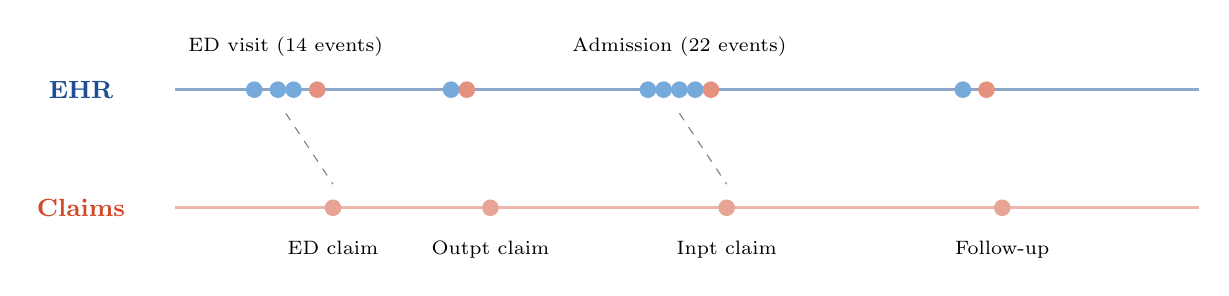
\begin{tikzpicture}[
    evt/.style={circle, minimum size=6pt, inner sep=0pt},
    lbl/.style={font=\scriptsize},
    timeline/.style={very thick}
]
% EHR Timeline
\node[font=\small\bfseries, columbia] at (-1.2, 1.5) {EHR};
\draw[timeline, columbia!50] (0, 1.5) -- (13, 1.5);

\node[evt, fill=columbialight] at (1.0, 1.5) {};
\node[evt, fill=columbialight] at (1.3, 1.5) {};
\node[evt, fill=columbialight] at (1.5, 1.5) {};
\node[evt, fill=columbiaaccent!60] at (1.8, 1.5) {};
\node[evt, fill=columbialight] at (3.5, 1.5) {};
\node[evt, fill=columbiaaccent!60] at (3.7, 1.5) {};
\node[evt, fill=columbialight] at (6.0, 1.5) {};
\node[evt, fill=columbialight] at (6.2, 1.5) {};
\node[evt, fill=columbialight] at (6.4, 1.5) {};
\node[evt, fill=columbialight] at (6.6, 1.5) {};
\node[evt, fill=columbiaaccent!60] at (6.8, 1.5) {};
\node[evt, fill=columbialight] at (10.0, 1.5) {};
\node[evt, fill=columbiaaccent!60] at (10.3, 1.5) {};

\node[lbl, above] at (1.4, 1.8) {ED visit (14 events)};
\node[lbl, above] at (6.4, 1.8) {Admission (22 events)};

% Claims Timeline
\node[font=\small\bfseries, columbiaaccent] at (-1.2, 0) {Claims};
\draw[timeline, columbiaaccent!40] (0, 0) -- (13, 0);

\node[evt, fill=columbiaaccent!50] at (2.0, 0) {};
\node[evt, fill=columbiaaccent!50] at (4.0, 0) {};
\node[evt, fill=columbiaaccent!50] at (7.0, 0) {};
\node[evt, fill=columbiaaccent!50] at (10.5, 0) {};

\node[lbl, below] at (2.0, -0.3) {ED claim};
\node[lbl, below] at (4.0, -0.3) {Outpt claim};
\node[lbl, below] at (7.0, -0.3) {Inpt claim};
\node[lbl, below] at (10.5, -0.3) {Follow-up};

% Arrows connecting
\draw[dashed, gray, thin] (1.4, 1.2) -- (2.0, 0.3);
\draw[dashed, gray, thin] (6.4, 1.2) -- (7.0, 0.3);
\end{tikzpicture}
\end{center}

\vspace{0.5em}
\textbf{Key insight:} The EHR shows 36+ individual events; claims condense this into 4 billing records.

\vspace{0.3em}
Claims data captures \textbf{what was billed for}, not \emph{what happened clinically}.
\end{frame}

\begin{frame}{When to Use Which?}
\begin{columns}[T]
\begin{column}{0.48\textwidth}
\textbf{Prefer EHR when:}
\begin{itemize}
    \item You need clinical details (lab values, vitals, medication doses)
    \item Temporal resolution matters (hourly ICU predictions)
    \item Clinical notes are important
    \item Single-institution study is acceptable
\end{itemize}
\end{column}
\begin{column}{0.48\textwidth}
\pause
\textbf{Prefer Claims when:}
\begin{itemize}
    \item You need population-level coverage
    \item You need cross-provider longitudinal data
    \item Utilization / cost is the outcome of interest
    \item Administrative codes are sufficient
\end{itemize}
\end{column}
\end{columns}

\vspace{1em}
\textbf{Increasingly:} Linked EHR--claims datasets combine the best of both worlds (e.g., All of Us, PCORnet).
\end{frame}

% ============================================================
% SECTION 7: STANDARDIZATION
% ============================================================




\section{Medical Coding Systems (Diagnoses)}

\begin{frame}{How do we represent medical observations?}
\begin{center}
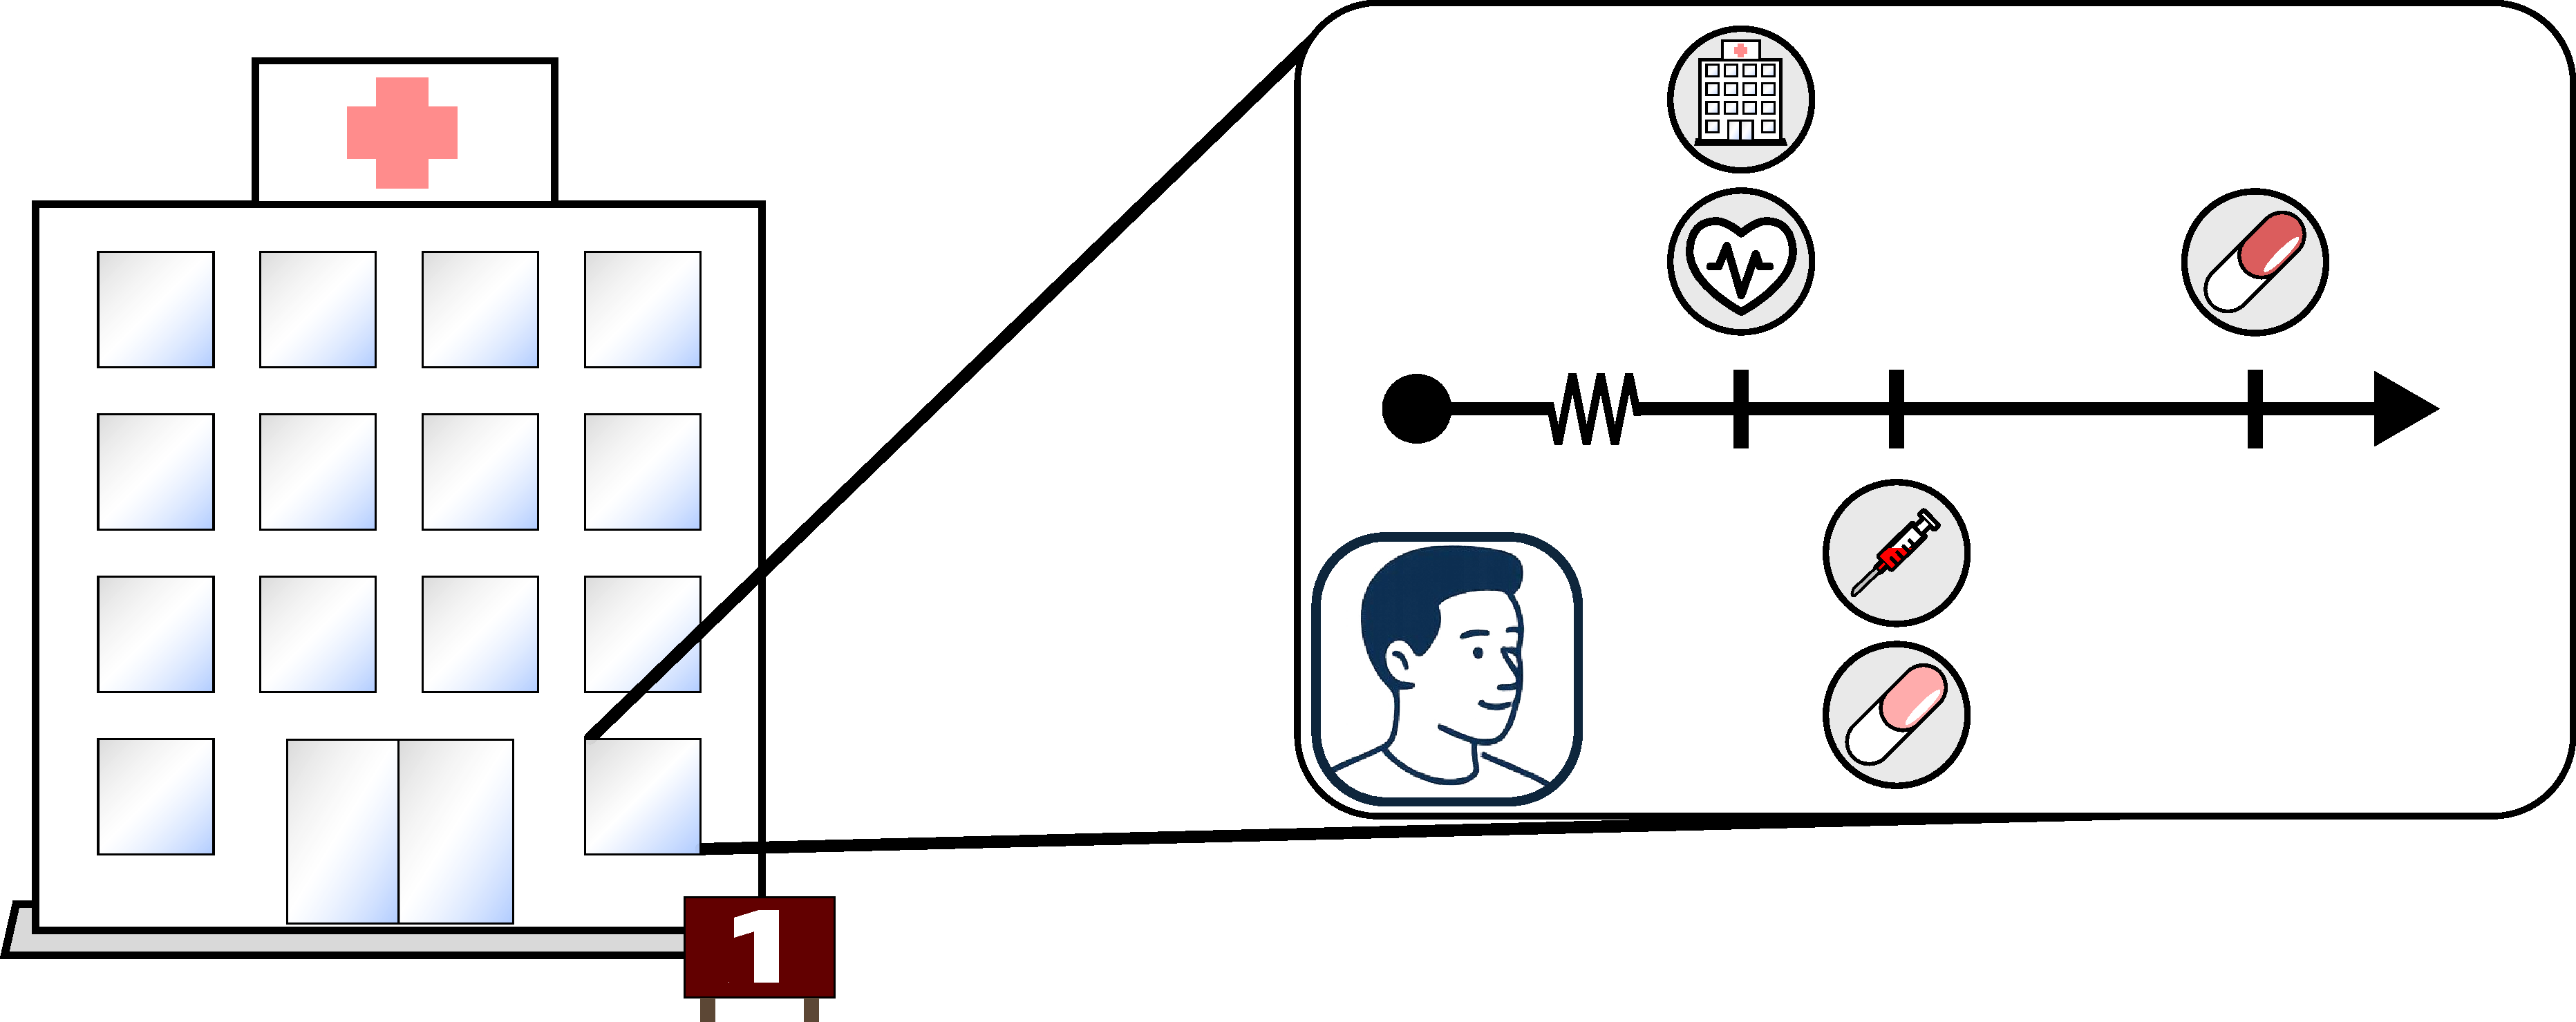
\includegraphics[width=0.65\textwidth]{figures/timeline.pdf}
\end{center}

\vspace{-0.3em}
\small
\begin{itemize}\setlength{\itemsep}{1pt}
    \item Each event has a \textbf{code} (ICD, LOINC, RxNorm, \ldots) and optionally a \textbf{value}
\end{itemize}
\end{frame}

\begin{frame}{Hierarchical Code Systems}
\textbf{Medical events are (often) coded in hierarchical vocabularies.}

\vspace{0.5em}
\begin{center}
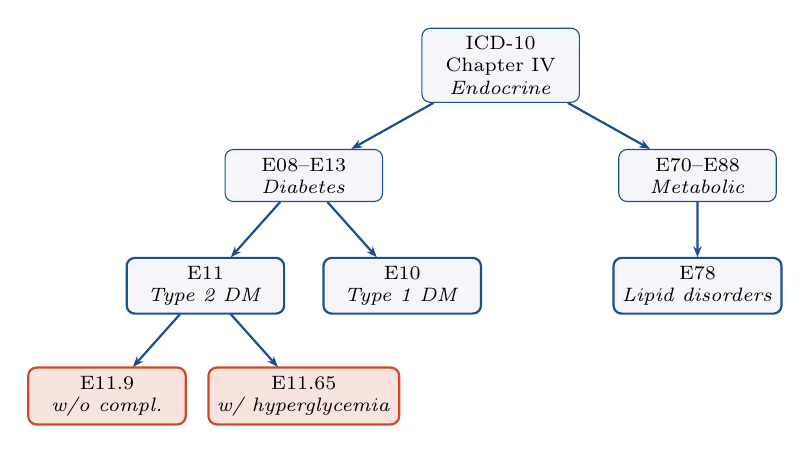
\begin{tikzpicture}[
    level distance=1.4cm,
    sibling distance=3.5cm,
    every node/.style={draw=columbia, rounded corners=3pt, fill=softbg,
                       font=\scriptsize, minimum width=2cm, align=center, inner sep=3pt},
    edge from parent/.style={draw=columbia, thick, -{Stealth[length=4pt]}},
    level 1/.style={sibling distance=5cm},
    level 2/.style={sibling distance=2.5cm},
]
\node {ICD-10\\Chapter IV\\\textit{Endocrine}}
    child { node {E08--E13\\\textit{Diabetes}}
        child { node {E11\\\textit{Type 2 DM}}
            child { node[fill=columbiaaccent!15, draw=columbiaaccent] {E11.9\\\textit{w/o compl.}} }
            child { node[fill=columbiaaccent!15, draw=columbiaaccent] {E11.65\\\textit{w/ hyperglycemia}} }
        }
        child { node {E10\\\textit{Type 1 DM}} }
    }
    child { node {E70--E88\\\textit{Metabolic}}
        child { node {E78\\\textit{Lipid disorders}} }
    };
\end{tikzpicture}
\end{center}

\vspace{0.5em}
\textbf{Modeling choice:} At which level do you define your features?\\
$\Rightarrow$ Finer coding granularity $=$ exponentially more features.
\end{frame}

\begin{frame}{Implications for ML}
\begin{block}{Consequences of Feature Dimensionality as a Design Choice}
\begin{enumerate}
    \item \textbf{Reproducibility:} Two studies on ``the same data'' with different code granularity are studying different problems
    \item \textbf{Curse of dimensionality:} Fine-grained codes $\Rightarrow$ sparse features $\Rightarrow$ more data needed
    \item \textbf{Information loss:} Coarse codes $\Rightarrow$ merge clinically distinct conditions
    \item \textbf{Sparse-data bias:} Over-stratification inflates ratio estimates (Rothman \& Mosquin, 2013)
\end{enumerate}
\end{block}

\vspace{0.5em}
\begin{itemize}
    \item Predicting ``any diabetes complication'' $\Rightarrow$ 3-character codes may suffice
    \item Predicting ``hyperosmolar coma'' specifically $\Rightarrow$ full ICD-10 codes needed
\end{itemize}
\end{frame}
% ── Problem 2: Ontology Issues ──
\begin{frame}{What Code Ontology to use?}
Multiple coding systems coexist, and they don't align cleanly:

\vspace{0.3em}
\begin{center}
\scriptsize
\begin{tabular}{lll}
\toprule
\textbf{System} & \textbf{Purpose} & \textbf{Problem} \\
\midrule
ICD-10-CM & Diagnosis billing & Changed from ICD-9 in 2015; cross-walks are many-to-many \\
SNOMED CT & Clinical documentation & Far more granular than ICD; no 1:1 mapping \\
LOINC & Lab test identification & Same test may have multiple LOINC codes across institutions \\
RxNorm & Medication naming & Generic vs.\ brand vs.\ ingredient-level conflicts \\
\bottomrule
\end{tabular}
\end{center}

\vspace{0.3em}
\textbf{Consequence:} ``Diabetes'' in Hospital A's EHR may correspond to a different set of codes than ``diabetes'' in Hospital B's EHR --- even if both use ICD-10.

\vspace{0.2em}
\textbf{ICD-9 $\to$ ICD-10 transition} (Oct 2015): A single ICD-9 code may map to 5--10 ICD-10 codes. Studies spanning this boundary face discontinuities.
\end{frame}

\begin{frame}{Even within an ontology, ambiguity persists!}
\textbf{Example: ICD-10 diabetes codes}

\vspace{0.2em}
\begin{center}
\scriptsize
\begin{tabular}{lp{5cm}p{4.5cm}}
\toprule
\textbf{Code} & \textbf{Description} & \textbf{Issue} \\
\midrule
E11.9 & T2DM without complications & Most commonly used (often a default) \\
E11.65 & T2DM with hyperglycemia & Clinically meaningful distinction \\
E11.69 & T2DM with other complication & ``Other'' is a catch-all \\
E13.9 & Other specified DM w/o compl. & Sometimes used for T2DM \\
R73.09 & Other abnormal glucose & Pre-diabetes? Early diabetes? \\
\bottomrule
\end{tabular}
\end{center}

\vspace{0.3em}
\textbf{Default-code problem:} Busy clinicians may select the first matching code (E11.9) regardless of complication status $\Rightarrow$ complication rates appear artificially low.

\vspace{0.2em}
\textbf{Upcoding:} Medicare risk adjustment may incentivize \emph{more severe} codes $\Rightarrow$ complication rates appear artificially high.

\end{frame}
\begin{frame}{Zipf's Law in Real Data (MIMIC-IV)}
\begin{center}
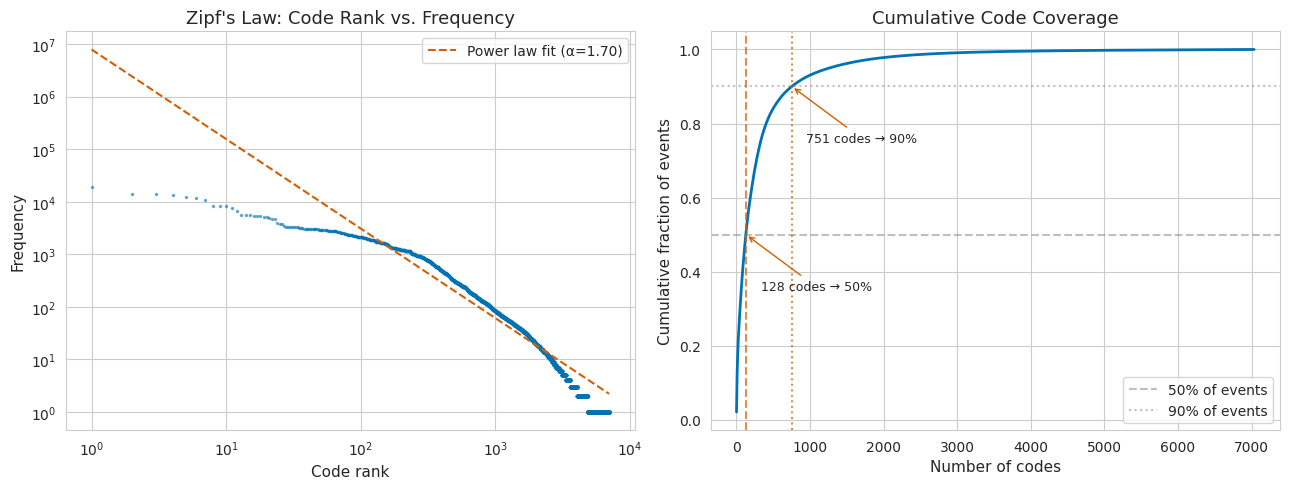
\includegraphics[width=0.92\textwidth]{figures/nb_zipf.png}
\end{center}

\vspace{-0.3em}
\scriptsize 128 codes (1.8\% of vocabulary) cover 50\% of all events. The long tail of 6,000+ rare codes is where the curse of dimensionality lives. Power-law exponent $\alpha = 1.70$. \textit{See Notebook 17, Section 3.}
\end{frame}

\section{Who is in the data?}

\begin{frame}{Health Data as a Collider}
\begin{center}
\Large
\textbf{All EHR data is conditioned on being in the health system.}
\end{center}
\vspace{0.5em}
\pause
Every patient in your dataset is there because they \emph{sought care}. This is a collider:
\begin{itemize}[<+->]
    \item Being sick $\to$ seeking care
    \item Being insured $\to$ seeking care
    \item Being health-conscious $\to$ seeking care
    \item Living near a hospital $\to$ seeking care
\end{itemize}
\pause
\vspace{0.5em}
This is exactly the celebrity example from the start of lecture --- but now the ``collider'' is \textbf{being in the EHR}.
\end{frame}
\begin{frame}{Berkson's Paradox in Real Data (MIMIC-IV)}
\begin{center}
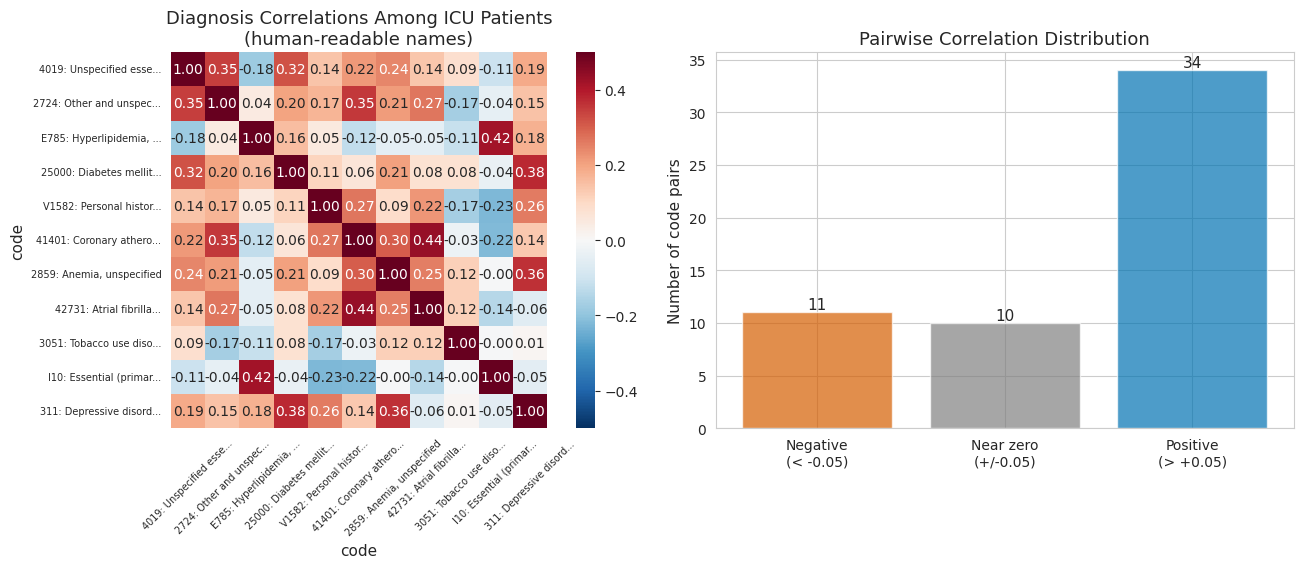
\includegraphics[width=0.95\textwidth]{figures/nb_berkson_corr.png}
\end{center}

\vspace{-0.3em}
\scriptsize Among 100 ICU patients, 11 diagnosis pairs show negative correlations. These conditions may be independent or positively correlated in the general population --- the negative associations are candidates for Berkson's bias from conditioning on ICU admission. \textit{See Notebook 17, Section 6.}
\end{frame}

\section{The Complexity of Health Data}


\begin{frame}{Why Health Data Is Hard for ML: A Roadmap}
\textbf{We'll use cohort selection examples to explore each of these challenges:}
\vspace{0.5em}
\begin{enumerate}[<+->]
    \item \textbf{Feature dimensionality} --- Zipf's law: a few codes are common, most are rare
    \item \textbf{Irregular sampling} --- events arrive at unpredictable times
    \item \textbf{Absent $\neq$ negative} --- missing data has meaning
    \item \textbf{Selection bias} --- who's in the data, and why?
    \item \textbf{Temporal complexity} --- left truncation, right censoring, gaps
    \item \textbf{Ontology fragmentation} --- same concept, different codes across systems
\end{enumerate}
\pause
\vspace{0.5em}
\textbf{Three running examples:}
\begin{description}
    \item[\color{columbia}\textbf{A}] T2DM 30-day readmission (chronic disease management)
    \item[\color{columbiaaccent}\textbf{B}] Sepsis in-hospital mortality (acute care)
    \item[\color{columbiagray}\textbf{C}] Statin adverse events (drug safety surveillance)
\end{description}
\end{frame}

\begin{frame}{Quick Check}
\begin{center}
\Large\textbf{Think--Pair--Share}
\end{center}

\vspace{0.8em}
If you're building a \textbf{diabetes prediction model}, would you use Chapter-level or Full-code-level ICD codes? Why?

\vspace{0.8em}
\textbf{Consider:}
\begin{itemize}
    \item How many training examples do you have?
    \item Does your model need to distinguish Type 1 from Type 2?
    \item What happens to rare codes in a logistic regression?
\end{itemize}
\end{frame}


% ============================================================
% SECTION 5: COHORT SELECTION
% ============================================================




% ============================================================
% SECTION: EXAMPLE TASK — COHORT SELECTION
% ============================================================
\section{Example Task: Cohort Selection}





\begin{frame}{Building a Study Cohort: Three Examples}
\begin{columns}[T]
\begin{column}{0.32\textwidth}
\begin{block}{\color{black}\textbf{A:} T2DM Readmission}
\small
\textbf{Population:} T2DM patients\\
\textbf{Outcome:} Readmitted within 30 days\\
\textbf{Data:} EHR or claims
\end{block}
\end{column}
\begin{column}{0.32\textwidth}
\begin{block}{\color{columbiaaccent}\textbf{B:} Sepsis Mortality}
\small
\textbf{Population:} Sepsis patients\\
\textbf{Outcome:} In-hospital death\\
\textbf{Data:} EHR (ICU)
\end{block}
\end{column}
\begin{column}{0.32\textwidth}
\begin{block}{\color{white}\textbf{C:} Statin Safety}
\small
\textbf{Population:} New statin users\\
\textbf{Outcome:} Rhabdomyolysis\\
\textbf{Data:} Claims
\end{block}
\end{column}
\end{columns}
\vspace{0.8em}
In standard ML, each is straightforward: define population, define outcome, extract features.
\vspace{0.3em}
\pause
\alert{In EHR/claims data, every one of these steps hides pitfalls.}
\vspace{0.2em}
For each problem below, we'll trace how it affects all three examples.
\end{frame}
\begin{frame}{Problem 1: Who Actually Has T2DM?}
\textbf{Option A: Require ICD code E11.x}
\begin{itemize}
    \item Misses undiagnosed patients (estimated 20\% of T2DM cases)
    \item Misses patients coded under E13 (``other specified diabetes'') or nonspecific codes
    \item Catches patients coded for billing reasons but clinically borderline
\end{itemize}

\vspace{0.5em}
\pause
\vspace{0.5em}
\textbf{Option B: Require E11.x OR A1c $\geq$ 6.5\% OR diabetes medication}
\begin{itemize}
    \item More sensitive, but: A1c may not be in claims data
    \item Metformin is also prescribed for PCOS --- false positives
    \item Lab thresholds vary by assay and institution
\end{itemize}

\vspace{0.8em}
\begin{center}
\colorbox{warnbg}{\parbox{0.85\textwidth}{\centering
\textbf{Fundamental issue:} The same clinical concept (``has T2DM'') maps to\\
different code combinations across institutions, coding practices, and time periods.
}}
\end{center}

\begin{center}\tiny
\textbf{\color{columbia}A:} E11.x? A1c $\geq$6.5\%? Metformin use? ~|~ \textbf{\color{columbiaaccent}B:} Sepsis-3 criteria? Culture + organ failure? ~|~ \textbf{\color{columbiagray}C:} First statin fill = new user?
\end{center}
\end{frame}

\begin{frame}{Problem 1b: ICD Codes Have Low Positive Predictive Value}
\textbf{Key finding} (Wei et al., \textit{JAMIA} 2016): Across 10 diseases, the PPV of a \emph{single} ICD code for identifying a patient who truly has the condition ranged from \textbf{0.06 to 0.71}.

\vspace{0.5em}
\begin{center}
\small
\begin{tabular}{lcc}
\toprule
\textbf{Evidence used} & \textbf{Average PPV} & \textbf{Average sensitivity} \\
\midrule
Single ICD code (no other support) & \textbf{0.37} & 0.67 \\
$\geq$2 ICD codes & 0.84 & Lower \\
ICD + clinical notes + medications & \textbf{0.91} & 0.59 \\
\bottomrule
\end{tabular}
\end{center}

\vspace{0.5em}
\textbf{Translation:} If you define your cohort as ``patients with $\geq$1 ICD code for T2DM,'' roughly \textbf{1 in 3} identified patients may not actually have the disease.

\vspace{0.3em}
\textbf{Best practice:} Combine ICD codes + clinical notes + lab values + medications for phenotyping. No single EHR component is sufficient alone.

\begin{center}\tiny
\textbf{\color{columbia}A:} Single E11.x code: PPV $\approx$0.37 ~|~ \textbf{\color{columbiaaccent}B:} Sepsis coding varies dramatically across sites ~|~ \textbf{\color{columbiagray}C:} Statin exposure well-captured in pharmacy claims
\end{center}
\end{frame}

% ── Problem 3: When Is a Patient "In" the Data? ──
\begin{frame}{Problem 3: When Is a Patient ``In'' Your Data?}
\begin{center}
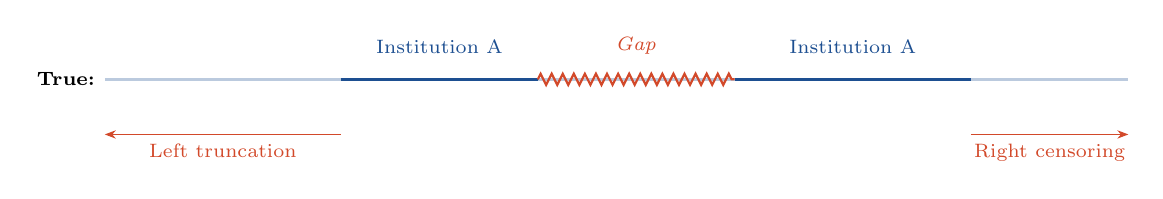
\begin{tikzpicture}[
    lbl/.style={font=\scriptsize},
    timeline/.style={very thick},
    gap/.style={decorate, decoration={zigzag, segment length=4pt, amplitude=2pt}}
]
% Full life timeline
\draw[timeline, columbia!30] (0,2) -- (13,2);
\node[lbl, left] at (0,2) {\textbf{True:}};

% Known data
\draw[timeline, columbia] (3,2) -- (5.5,2);
\draw[timeline, columbia] (8,2) -- (11,2);

% Gap markers
\draw[gap, columbiaaccent, thick] (5.5,2) -- (8,2);

% Labels
\node[lbl, above, columbia] at (4.25, 2.2) {Institution A};
\node[lbl, above, columbia] at (9.5, 2.2) {Institution A};
\node[lbl, above, columbiaaccent] at (6.75, 2.2) {\textit{Gap}};

% Brackets
\draw[{Stealth[length=4pt]}-, columbiaaccent] (0, 1.3) -- (3, 1.3)
    node[midway, below, font=\scriptsize\color{columbiaaccent}] {Left truncation};
\draw[-{Stealth[length=4pt]}, columbiaaccent] (11, 1.3) -- (13, 1.3)
    node[midway, below, font=\scriptsize\color{columbiaaccent}] {Right censoring};
\end{tikzpicture}
\end{center}

\small
\begin{description}\setlength{\itemsep}{2pt}
    \item[Left truncation:] Patient enters \emph{your} system. A ``new'' diagnosis may be a 10-year history from another hospital.
    \item[Mid-record gaps:] Patient switches insurer or seeks care elsewhere $\Rightarrow$ gap = \textbf{unobserved events}.
    \item[Right censoring:] Patient leaves. No readmission in your data $\neq$ no readmission anywhere.
\end{description}

\begin{center}\tiny
\textbf{\color{columbia}A:} Prior A1c history invisible after transfer ~|~ \textbf{\color{columbiaaccent}B:} Prior ICU stays at other hospitals unknown ~|~ \textbf{\color{columbiagray}C:} Statin use before enrollment period invisible
\end{center}
\end{frame}

\begin{frame}{Problem 3b: Membership and Eligibility Ambiguity}
\textbf{In claims data:} You only observe patients during periods of \textbf{plan membership}.

\vspace{0.5em}
\begin{center}
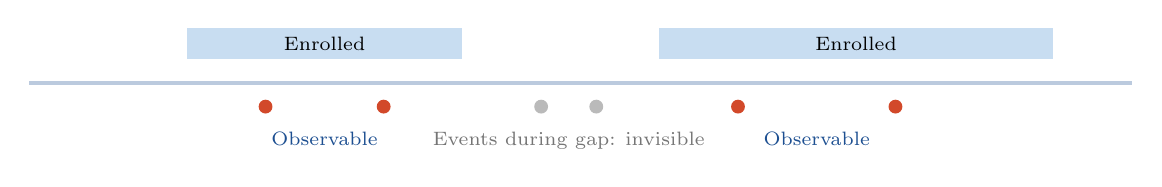
\begin{tikzpicture}[
    lbl/.style={font=\scriptsize},
    timeline/.style={very thick}
]
\draw[timeline, columbia!30] (0,0) -- (14,0);
% Membership bar
\fill[columbialight!40] (2, 0.3) rectangle (5.5, 0.7);
\fill[columbialight!40] (8, 0.3) rectangle (13, 0.7);
\node[lbl] at (3.75, 0.5) {Enrolled};
\node[lbl] at (10.5, 0.5) {Enrolled};

% Events
\node[circle, fill=columbiaaccent, minimum size=5pt, inner sep=0pt] at (3, -0.3) {};
\node[circle, fill=columbiaaccent, minimum size=5pt, inner sep=0pt] at (4.5, -0.3) {};
\node[circle, fill=columbiagray!50, minimum size=5pt, inner sep=0pt] at (6.5, -0.3) {};
\node[circle, fill=columbiagray!50, minimum size=5pt, inner sep=0pt] at (7.2, -0.3) {};
\node[circle, fill=columbiaaccent, minimum size=5pt, inner sep=0pt] at (9, -0.3) {};
\node[circle, fill=columbiaaccent, minimum size=5pt, inner sep=0pt] at (11, -0.3) {};

\node[lbl, below] at (6.85, -0.5) {\color{columbiagray}Events during gap: invisible};
\node[lbl, below] at (3.75, -0.5) {\color{columbia}Observable};
\node[lbl, below] at (10, -0.5) {\color{columbia}Observable};
\end{tikzpicture}
\end{center}

\vspace{0.5em}
\textbf{Pre-membership history:} Patient joins plan with existing T2DM.
Their ``first'' diabetes code in your data isn't truly their first.

\vspace{0.3em}
\textbf{Post-membership follow-up:} Patient leaves plan 15 days after discharge.
You see no readmission --- is that a \textbf{true negative} or \textbf{censored}?

\vspace{0.3em}
\textbf{Rule of thumb:} Require a ``clean enrollment period'' (e.g., 6--12 months continuous enrollment before index date) --- but this creates selection bias toward stable, insured patients.

\begin{center}\tiny
\textbf{\color{columbia}A:} Readmission window starts at discharge --- need clean enrollment ~|~ \textbf{\color{columbiaaccent}B:} Transferred sepsis patients: which ICU ``owns'' the outcome? ~|~ \textbf{\color{columbiagray}C:} Gaps in pharmacy coverage = missing fills, not non-adherence
\end{center}
\end{frame}

\begin{frame}{Observation Windows in Real Data (MIMIC-IV)}
\begin{center}
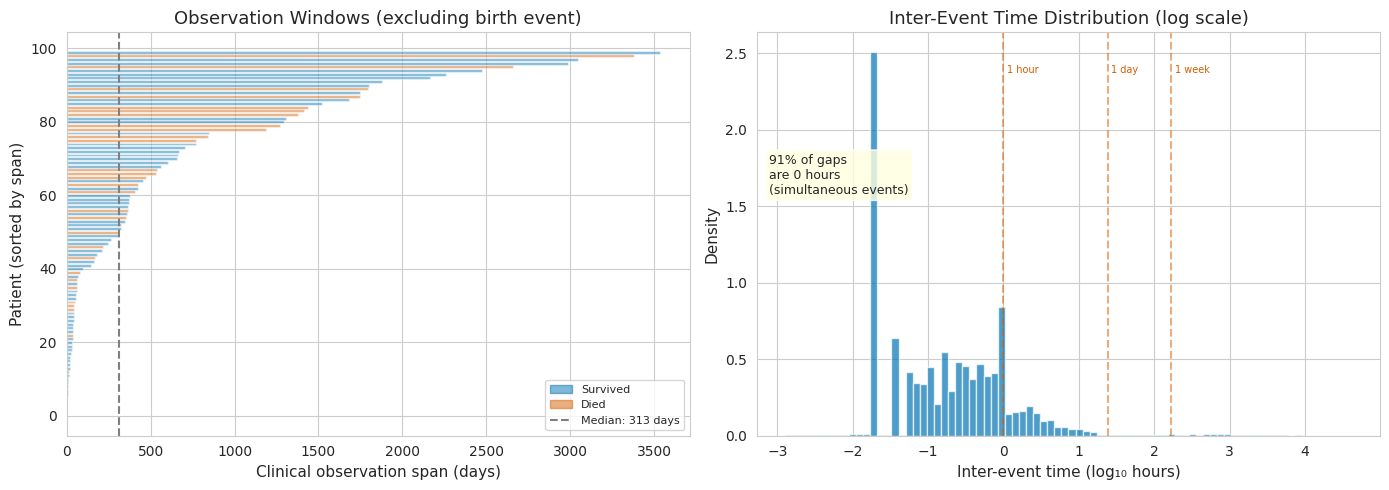
\includegraphics[width=0.95\textwidth]{figures/nb_censoring.png}
\end{center}

\vspace{-0.3em}
\scriptsize \textbf{Left:} Each bar is one patient's clinical observation window (excluding birth event). Died patients in orange. \textbf{Right:} Inter-event times on log scale --- 91\% are simultaneous (ICU is dense!). Reference lines at 1 hour, 1 day, 1 week. \textit{See Notebook 17, Section 8.}
\end{frame}

% ── Problem 4: Coverage Gaps ──
\begin{frame}{Problem 4: Not All Care Is Captured}
\begin{columns}[T]
\begin{column}{0.48\textwidth}
\textbf{EHR data} misses:
\begin{itemize}
    \item Specialist visits at a different hospital
    \item Urgent care / retail clinic visits
    \item Behavioral health (often separate systems)
    \item OTC medications, supplements
    \item Care received while traveling
\end{itemize}
\end{column}
\begin{column}{0.48\textwidth}
\pause
\textbf{Claims data} misses:
\begin{itemize}
    \item Cash-pay services (cosmetic, mental health)
    \item Services during coverage gaps
    \item Denied / rejected claims
    \item Non-medical determinants (housing, food)
\end{itemize}
\end{column}
\end{columns}

\vspace{0.5em}
\alert{Neither source gives you a complete picture of a patient's health.}\\
This is not ``missing at random'' --- it's systematically related to socioeconomic status, geography, and care-seeking behavior.

\begin{center}\tiny
\textbf{\color{columbia}A:} Outpatient diabetes care at another clinic invisible ~|~ \textbf{\color{columbiaaccent}B:} Transfer from outside hospital: missing early course ~|~ \textbf{\color{columbiagray}C:} OTC supplements, cash-pay statins not in claims
\end{center}
\end{frame}

% ── Problem 5: Informative Observation ──
\begin{frame}{Problem 5: Sicker Patients Generate More Data}
\begin{columns}[T]
\begin{column}{0.55\textwidth}
In standard ML, we assume:
\[
    \text{Observation times} \perp\!\!\!\perp \text{Outcome} \quad \text{(are independent of)}
\]
In EHR, this is \textbf{almost always violated}.

\vspace{0.5em}
\textbf{Why?}
\begin{itemize}
    \item Sicker patients visit more often
    \item Clinicians order more tests when concerned
    \item ICU: continuous monitoring; outpatient: yearly
\end{itemize}

\vspace{0.5em}
\textbf{Consequence:}\\
``\# of lab tests'' is one of the strongest predictors of readmission --- not because tests cause readmission.
\end{column}
\begin{column}{0.42\textwidth}
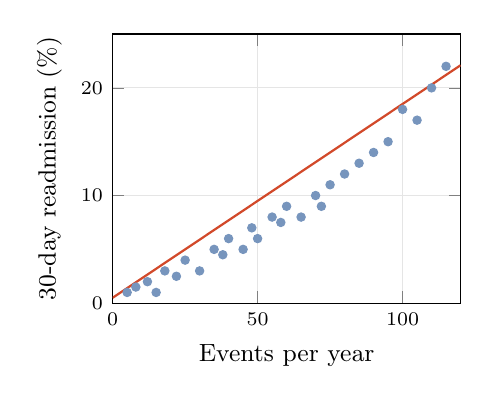
\begin{tikzpicture}
\begin{axis}[
    width=6cm, height=5cm,
    xlabel={Events per year},
    ylabel={30-day readmission (\%)},
    xlabel style={font=\small},
    ylabel style={font=\small},
    tick label style={font=\scriptsize},
    ymin=0, ymax=25,
    xmin=0, xmax=120,
    grid=major,
    grid style={gray!20},
]
\addplot[only marks, mark=*, mark size=1.5pt, columbia!60] coordinates {
    (5,1) (8,1.5) (12,2) (15,1) (18,3) (22,2.5)
    (25,4) (30,3) (35,5) (38,4.5) (40,6) (45,5)
    (48,7) (50,6) (55,8) (58,7.5) (60,9) (65,8)
    (70,10) (72,9) (75,11) (80,12) (85,13) (90,14)
    (95,15) (100,18) (105,17) (110,20) (115,22)
};
\addplot[thick, columbiaaccent, domain=0:120, samples=50]
    {0.18*x + 0.5};
\end{axis}
\end{tikzpicture}
\end{column}
\end{columns}

\vspace{0.2em}
\scriptsize \textit{``Informative observation'' (who gets measured more) $\neq$ ``informative missingness'' (what doesn't get measured). Both violate standard ML assumptions.}

\begin{center}\tiny
\textbf{\color{columbia}A:} Frequent flyers have more DM codes = easier to find ~|~ \textbf{\color{columbiaaccent}B:} Sicker sepsis patients have more labs = richer features ~|~ \textbf{\color{columbiagray}C:} Patients with AEs generate more claims = detection bias
\end{center}
\end{frame}

% ── Problem 6: Immortal Time Bias ──
\begin{frame}{Problem 6: Immortal Time Bias}
\begin{center}
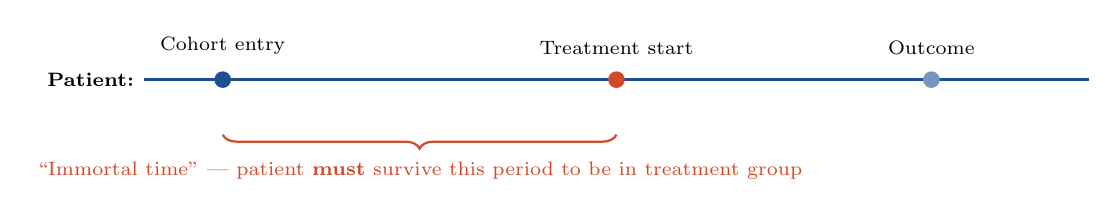
\begin{tikzpicture}[
    lbl/.style={font=\scriptsize},
    timeline/.style={very thick}
]
% Patient timeline
\draw[timeline, columbia] (0,1.5) -- (12,1.5);
\node[lbl, left] at (0,1.5) {\textbf{Patient:}};

% Markers
\node[circle, fill=columbia, minimum size=6pt, inner sep=0pt] at (1,1.5) {};
\node[lbl, above] at (1, 1.7) {Cohort entry};

\node[circle, fill=columbiaaccent, minimum size=6pt, inner sep=0pt] at (6,1.5) {};
\node[lbl, above] at (6, 1.7) {Treatment start};

\node[circle, fill=columbia!60, minimum size=6pt, inner sep=0pt] at (10,1.5) {};
\node[lbl, above] at (10, 1.7) {Outcome};

% Immortal time bracket
\draw[decorate, decoration={brace, amplitude=5pt, mirror}, columbiaaccent, thick]
    (1, 0.8) -- (6, 0.8) node[midway, below=6pt, font=\scriptsize\color{columbiaaccent}] {``Immortal time'' --- patient \textbf{must} survive this period to be in treatment group};
\end{tikzpicture}
\end{center}

\vspace{0.5em}
\textbf{The trap:} If you compare ``patients who received Drug X'' vs.\ ``patients who didn't,'' treated patients are \emph{guaranteed} to have survived long enough to receive the drug.

\vspace{0.3em}
\textbf{For our T2DM cohort:} If we require ``started on metformin after diagnosis,'' patients who died or were readmitted before starting metformin are excluded $\Rightarrow$ treatment group looks artificially healthier.

\vspace{0.5em}
\textbf{Solutions:} Landmark analysis, time-varying covariates, target trial emulation.

\begin{center}\tiny
\textbf{\color{columbia}A:} Must survive to discharge $\to$ readmission possible ~|~ \textbf{\color{columbiaaccent}B:} Must survive to receive antibiotics ~|~ \textbf{\color{columbiagray}C:} Must survive long enough on statin to develop AE
\end{center}
\end{frame}

% ── Problem 7: The Fundamental Ambiguity ──

\begin{frame}{The Fundamental Ambiguity}
\begin{center}
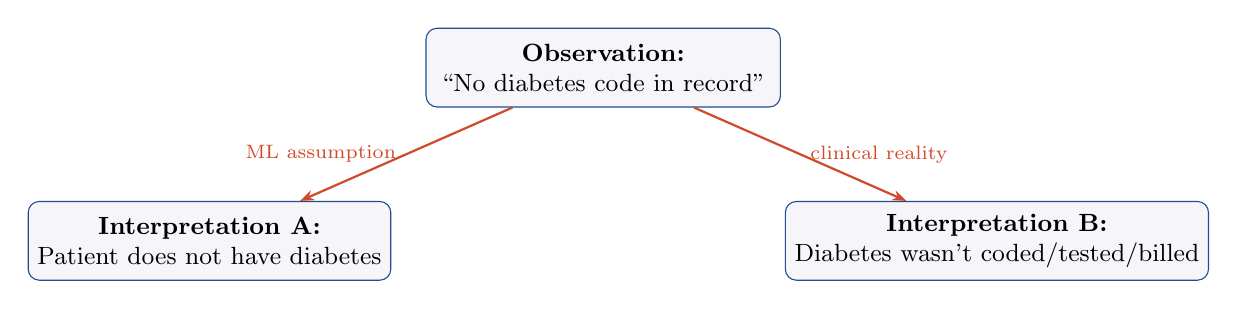
\begin{tikzpicture}[
    box/.style={draw=columbia, fill=softbg, rounded corners=4pt,
                minimum width=4.5cm, minimum height=1cm, align=center, font=\small},
    arr/.style={-{Stealth[length=5pt]}, thick, columbiaaccent}
]
\node[box] (obs) at (0, 0) {\textbf{Observation:}\\``No diabetes code in record''};
\node[box] (int1) at (-5, -2.2) {\textbf{Interpretation A:}\\Patient does not have diabetes};
\node[box] (int2) at (5, -2.2) {\textbf{Interpretation B:}\\Diabetes wasn't coded/tested/billed};

\draw[arr] (obs) -- (int1) node[midway, left, font=\scriptsize\color{columbiagray}] {ML assumption};
\draw[arr] (obs) -- (int2) node[midway, right, font=\scriptsize\color{columbiagray}] {clinical reality};
\end{tikzpicture}
\end{center}

\vspace{0.3em}
\textbf{``Absent'' $\neq$ ``Not measured'' $\neq$ ``Negative''}
\begin{itemize}[<+->]
    \item No lab result $\Rightarrow$ test wasn't ordered (not: result was normal)
    \item No diagnosis code $\Rightarrow$ condition wasn't billed for (not: condition absent)
    \item No medication $\Rightarrow$ wasn't prescribed in \emph{this system} (not: patient isn't taking it)
\end{itemize}

\begin{center}\tiny
\textbf{\color{columbia}A:} No A1c $\Rightarrow$ not ordered, not normal ~|~ \textbf{\color{columbiaaccent}B:} No blood culture $\Rightarrow$ not suspected, not ruled out ~|~ \textbf{\color{columbiagray}C:} No statin refill $\Rightarrow$ stopped, switched, or cash-pay
\end{center}
\end{frame}


\begin{frame}{Summary: A Taxonomy of Cohort Selection Pitfalls}
\begin{center}
\scriptsize
\begin{tabular}{p{3cm}p{3.5cm}p{5.5cm}}
\toprule
\textbf{Problem} & \textbf{Mechanism} & \textbf{Consequence for ML} \\
\midrule
Ambiguous case definition & Codes $\neq$ clinical reality & Noisy labels, variable prevalence \\
Low code PPV & Code $\neq$ disease & Noisy labels even with ``clean'' codes \\
Ontology fragmentation & Multiple coding systems & Cross-site non-comparability \\
Left truncation & Prior history invisible & Missing baseline severity \\
Mid-record gaps & Different system/plan & False ``event-free'' periods \\
Right censoring & Patient leaves data & Biased outcome measurement \\
Coverage gaps & Not all care captured & Systematic feature missingness \\
Informative observation & Sick $\to$ more data & Confounded feature counts \\
Immortal time bias & Must survive to be treated & Inflated treatment benefits \\
Upcoding & Financial incentives & Distorted disease severity \\
\alert{Berkson's bias} & \alert{Conditioned on being in data} & \alert{Spurious associations} \\
\bottomrule
\end{tabular}
\end{center}

\vspace{0.2em}
\textbf{Recall:} Which of these are instances of Berkson's Paradox from the start of lecture?
\end{frame}

\section{Standardization \& Interoperability}



\begin{frame}{The Reproducibility Problem}
\textbf{Today:} Most health AI studies use single-institution data with custom preprocessing.

\vspace{0.5em}
\textbf{Result:}
\begin{itemize}
    \item Models don't transfer across hospitals
    \item Results can't be independently verified
    \item Code is institution-specific and unreusable
\end{itemize}

\vspace{0.5em}
\textbf{The standardization response:}

\vspace{0.2em}
\begin{center}
\small
\begin{tabular}{lp{9.5cm}}
\toprule
\textbf{Standard} & \textbf{Purpose} \\
\midrule
OMOP CDM & Common data model for observational health data; maps local codes to standard vocabularies \\
FHIR & Interoperability standard for real-time data exchange between systems \\
MEDS & ML-focused event-stream standard for EHR data \\
\bottomrule
\end{tabular}
\end{center}
\end{frame}


\begin{frame}{MEDS: A Minimal Format for ML}
\begin{center}
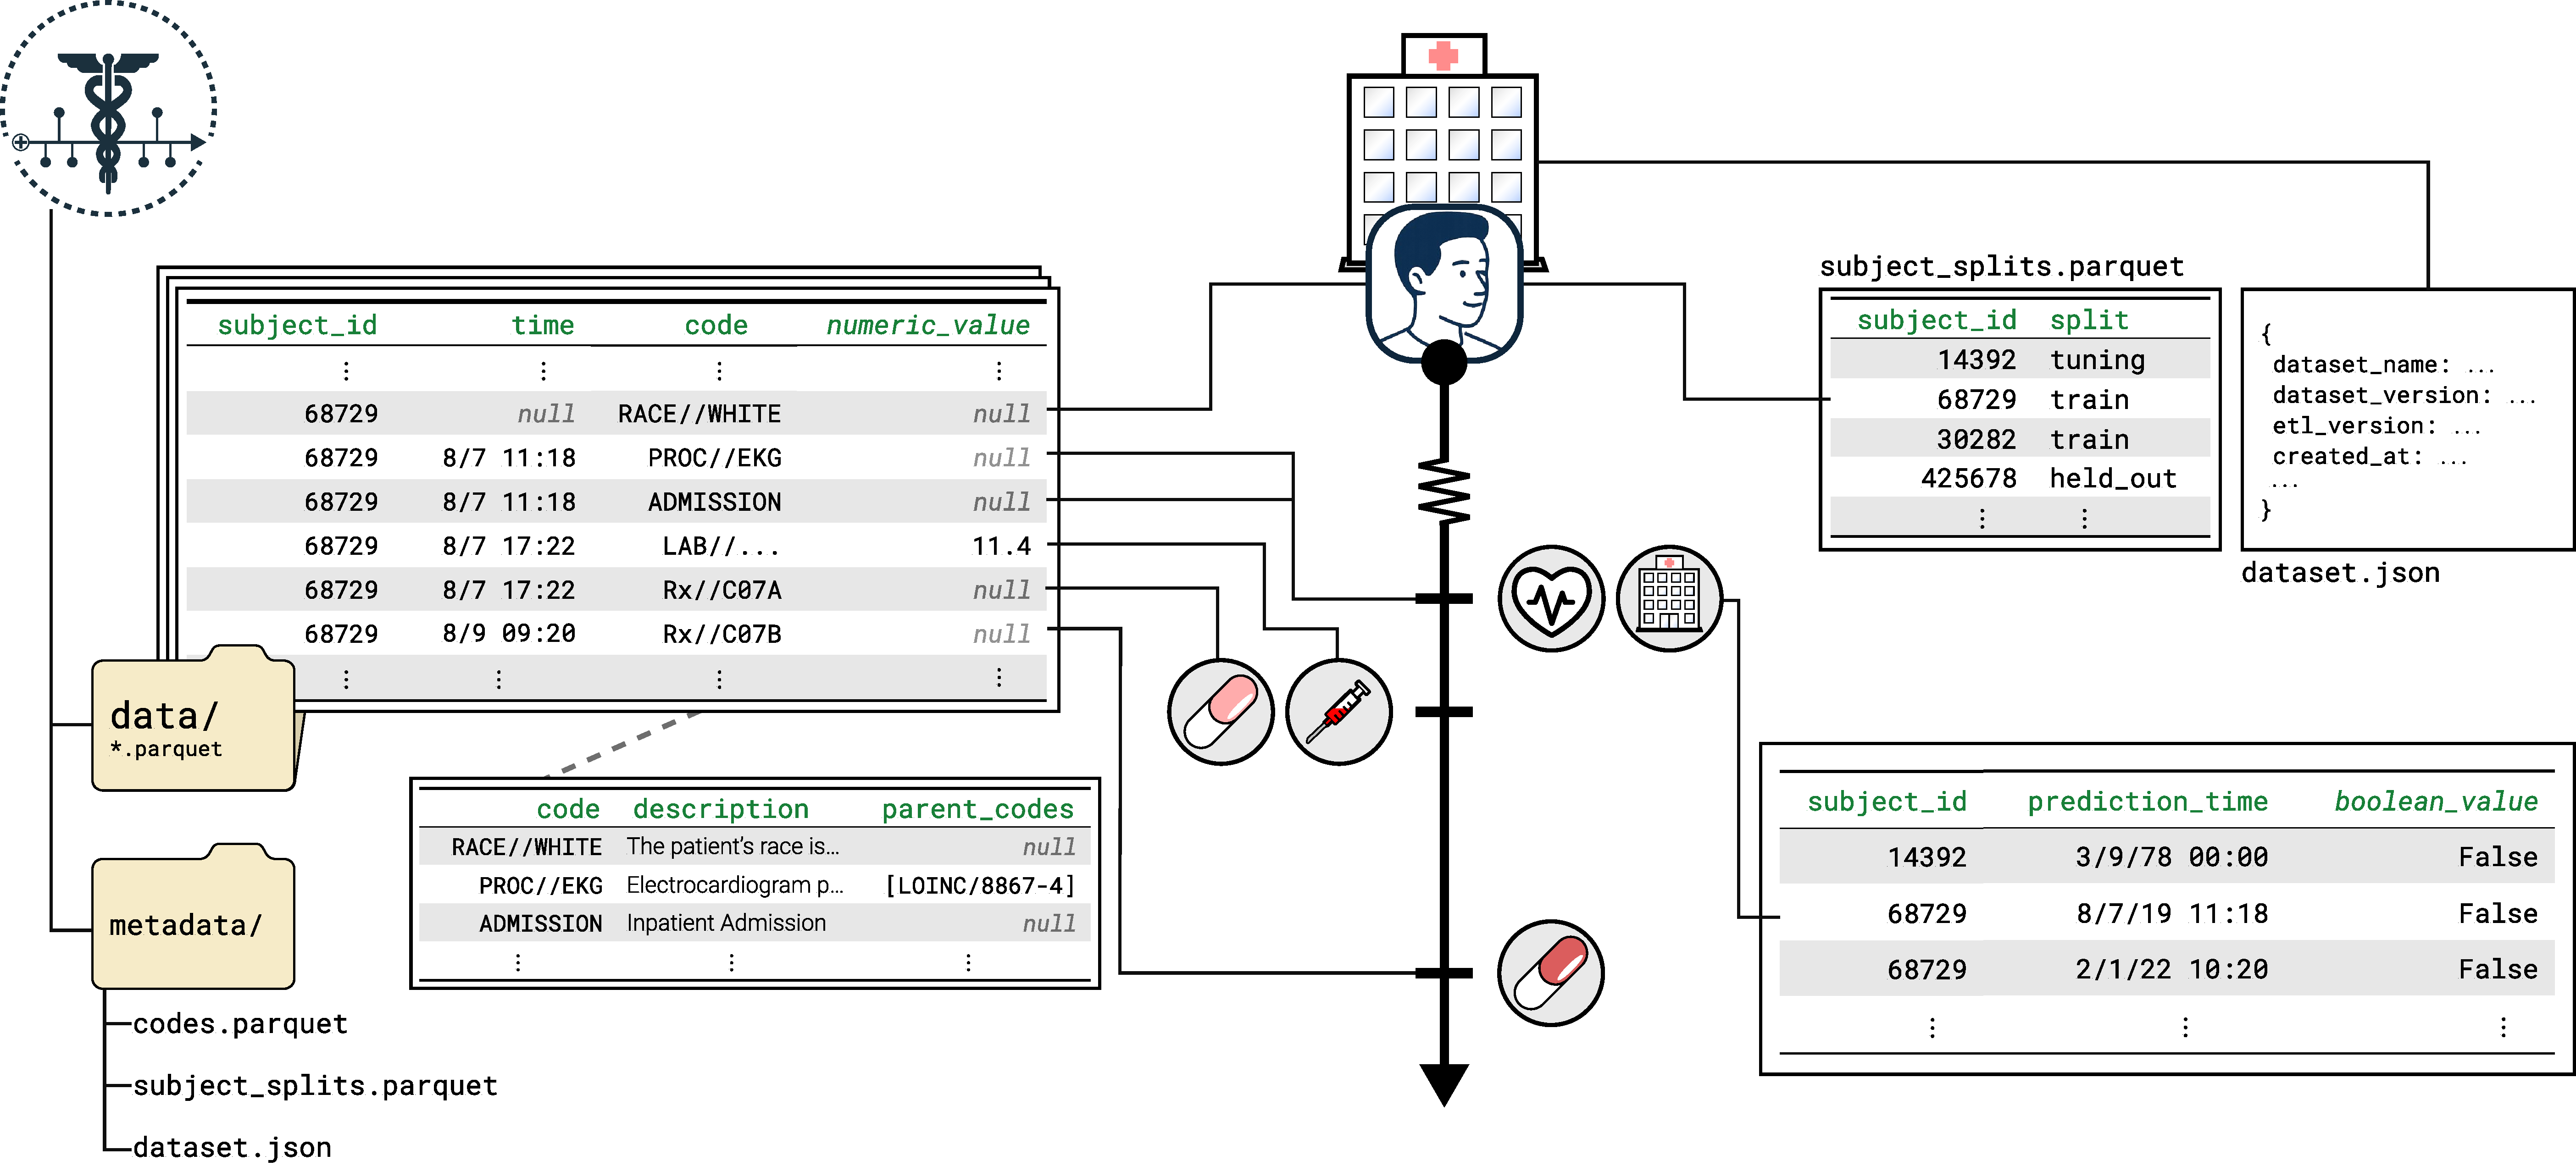
\includegraphics[width=0.82\textwidth]{figures/MEDS_schema.pdf}
\end{center}

\vspace{-0.2em}
\scriptsize Each patient's record is a simple table: (subject\_id, time, code, numeric\_value). The code column is unconstrained --- any coding system works.
\end{frame}


\begin{frame}{OMOP CDM: The Most Widely Adopted Standard}
\begin{center}
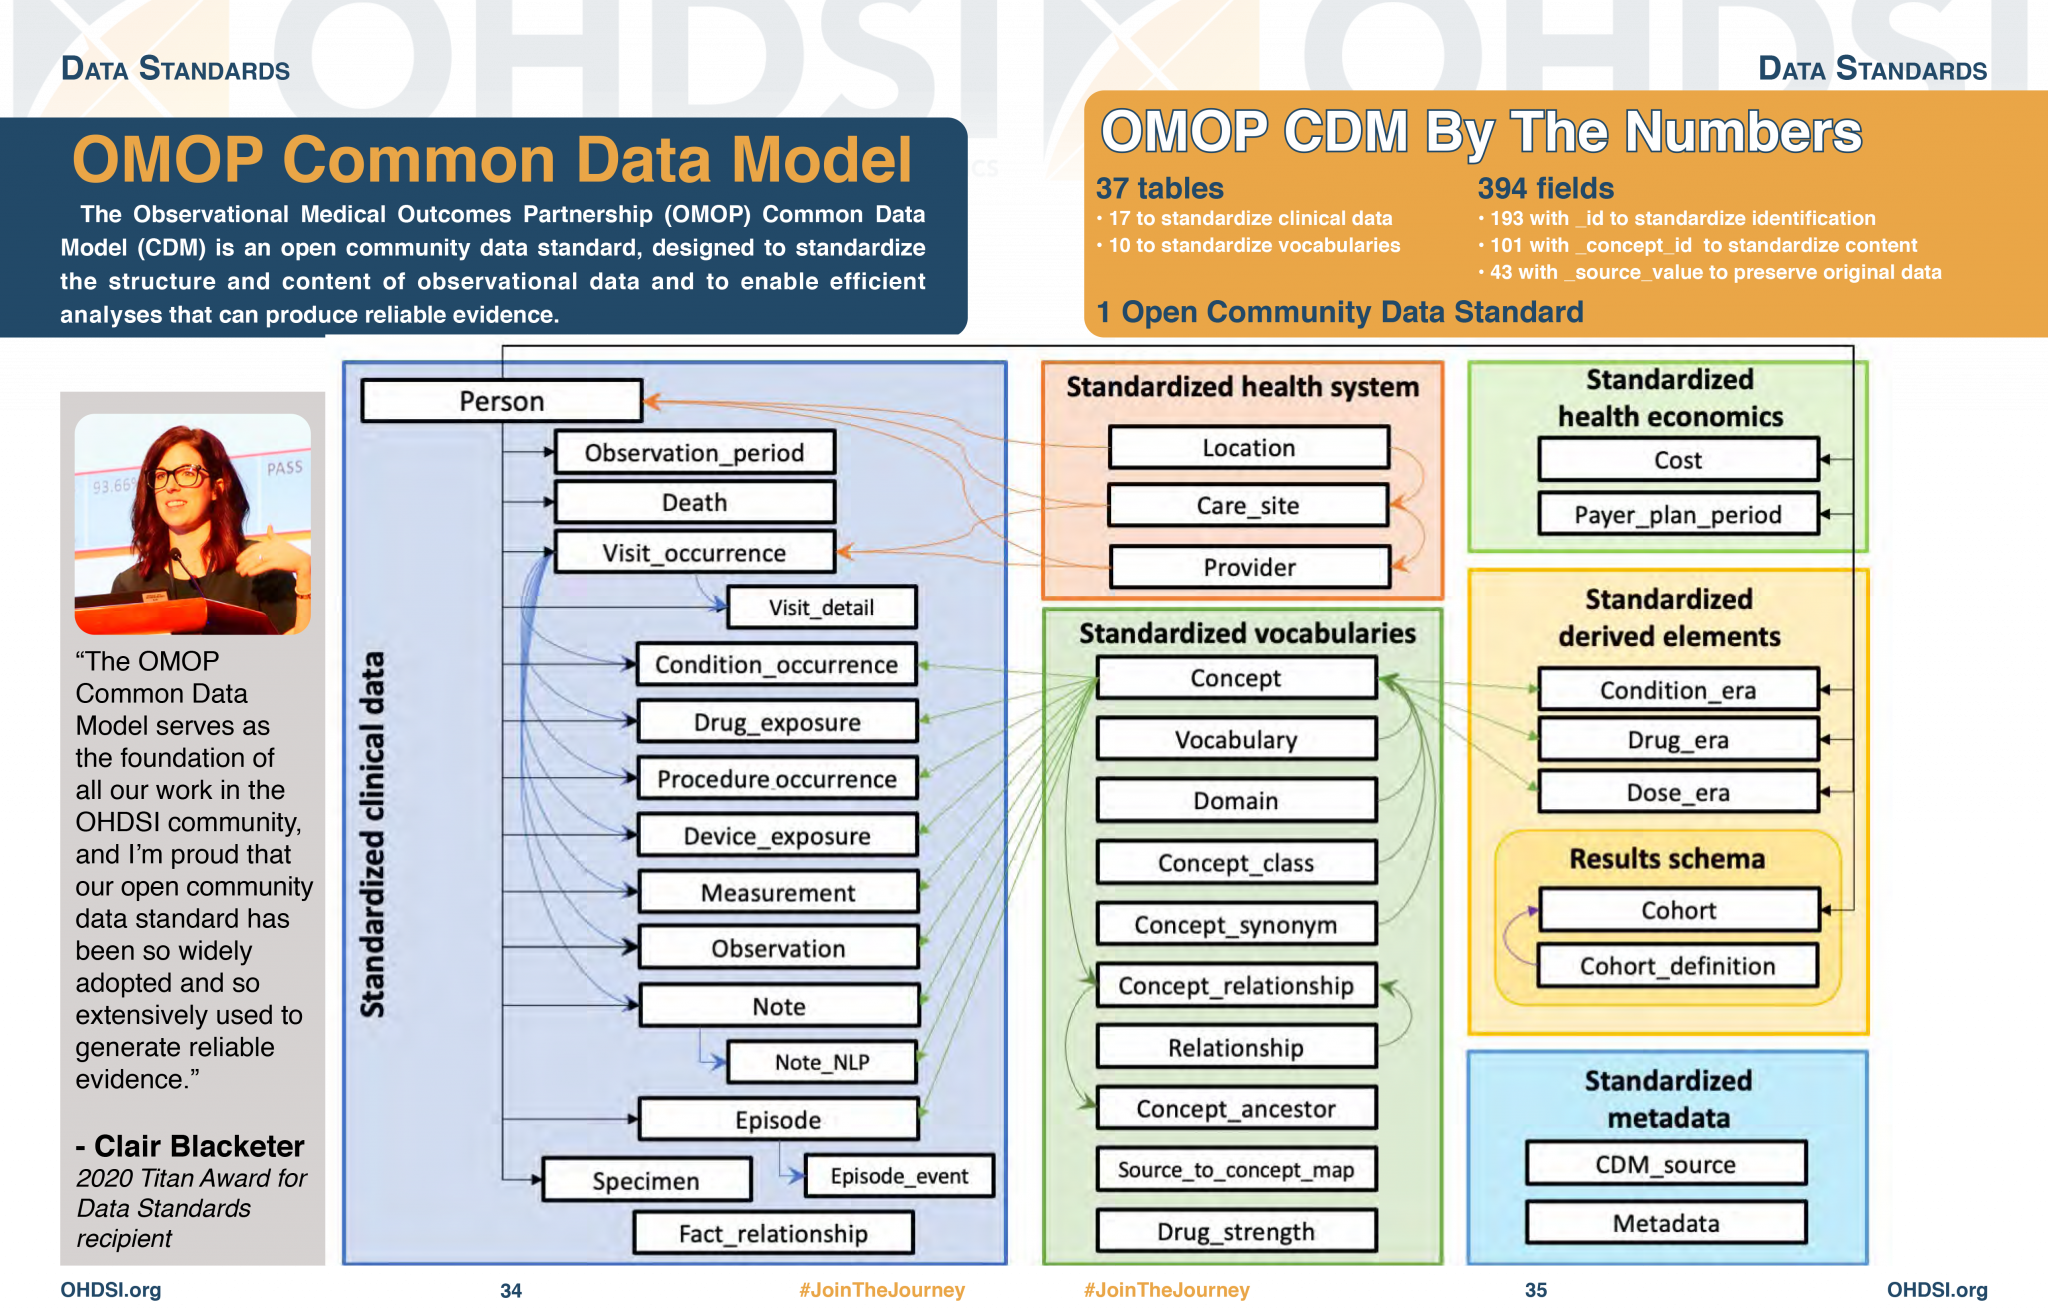
\includegraphics[width=0.82\textwidth]{figures/omop_cdm_schema.png}
\end{center}

\vspace{-0.2em}
\scriptsize OMOP CDM: 37 tables, 394 fields. Used by hundreds of institutions worldwide via OHDSI. Far more comprehensive than MEDS --- designed for observational research, not specifically ML pipelines.
\end{frame}


% ============================================================

\begin{frame}{One Approach: Tabularizing the Event Stream}
\textbf{Traditional ML models} require fixed-length feature vectors. One common approach is to \emph{tabularize} the event stream:

\vspace{0.3em}
\begin{center}
\scriptsize
\begin{tabular}{lll}
\toprule
\textbf{time} & \textbf{code} & \textbf{value} \\
\midrule
Day 0 & E11.9 (T2DM) & -- \\
Day 0 & LAB/A1c & 7.2 \\
Day 14 & RX/metformin & -- \\
Day 45 & LAB/A1c & 6.8 \\
Day 45 & E78.0 (hyperlipid.) & -- \\
\bottomrule
\end{tabular}
\quad$\xrightarrow{\text{tabularize}}$\quad
\begin{tabular}{lr}
\toprule
\textbf{Feature} & \textbf{Value} \\
\midrule
has\_E11 & 1 \\
has\_E78 & 1 \\
n\_events & 5 \\
A1c\_mean & 7.0 \\
A1c\_last & 6.8 \\
n\_meds & 1 \\
span\_days & 45 \\
\bottomrule
\end{tabular}
\end{center}

\vspace{0.3em}
\alert{Every one of these choices discards information} --- temporal ordering, event co-occurrence within encounters, and the raw event stream itself.

\vspace{0.3em}
\textbf{Alternative:} Deep learning models (Transformers, RNNs) can operate directly on the event stream without tabularization. We'll return to this in later lectures.
\end{frame}

% ============================================================






\section{Summary}


\begin{frame}{Today's Takeaways}
\begin{enumerate}
    \item \textbf{EHR data is unlike any standard ML data type} --- irregularly sampled, variably structured, generated as a byproduct of care
    \item \textbf{Claims data} reflects billing, not clinical care --- different features, different biases, population-level breadth
    \item \textbf{Cohort selection} illustrates key challenges: ambiguous definitions, low PPV, ontology fragmentation, truncation, censoring, informative observation
    \item \textbf{Berkson's Paradox:} EHR data is conditioned on seeking care --- every association may be distorted by selection
    \item \textbf{Standardization} (OMOP, FHIR, MEDS) enables reproducibility
\end{enumerate}
\vspace{0.3em}
\textbf{Notebook:} \texttt{nb17\_ehr\_claims.ipynb} --- explore these concepts with real MIMIC-IV data in MEDS format.
\end{frame}
\begin{frame}[standout]
    Questions?
\end{frame}

% ============================================================
% APPENDIX
% ============================================================
\appendix



\appendix


\appendix

\begin{frame}{Recall: Temporal Point Processes}
A \textbf{temporal point process} (TPP) is a stochastic model for a sequence of events in continuous time.

\vspace{0.3em}
\textbf{Intuition:} Think of it as modeling ``how many events per hour would we expect \emph{right now}, given everything that's already happened to this patient?''

\vspace{0.5em}
\textbf{Formal definition:} A realization is a sequence of event times and marks:
\[
    \mathcal{H} = \{(t_1, m_1),\; (t_2, m_2),\; \ldots,\; (t_N, m_N)\}
    \quad\text{where}\quad t_1 < t_2 < \cdots < t_N
\]

\vspace{0.3em}
Characterized by a \textbf{conditional intensity function}:
\[
    \lambda^*(t, m) = \lim_{\Delta t \to 0}
    \frac{\Pr(\text{event of type } m \text{ in } [t, t+\Delta t) \mid \mathcal{H}_t)}{\Delta t}
\]

\vspace{0.5em}
\textbf{Contrast with regular timeseries:}
\begin{itemize}
    \item Regular TS: observations at fixed intervals $(x_1, x_2, \ldots, x_T)$
    \item TPP: observations at \emph{random} times --- the \emph{timing itself} is part of the data
\end{itemize}
\end{frame}

\begin{frame}{Mapping EHR $\to$ TPP}
\begin{center}
\begin{tabular}{lll}
\toprule
\textbf{TPP Concept} & \textbf{EHR Realization} & \textbf{Example} \\
\midrule
Event time $t_i$ & Timestamp of clinical event & 2024-03-15 14:32 \\
Mark $m_i$ & Clinical code + value & ICD: E11.9 (T2DM) \\
History $\mathcal{H}_t$ & All prior events for patient & Full record to date \\
Intensity $\lambda^*(t)$ & Rate of clinical events & Higher during hospitalization \\
Inter-event time & Gap between encounters & 3 days vs.\ 6 months \\
\bottomrule
\end{tabular}
\end{center}

\vspace{0.8em}
\begin{alertblock}{Where the mapping breaks}
\begin{enumerate}
    \item \textbf{Observation process is informative} --- sicker patients generate more events
    \item \textbf{Multiple simultaneous events} --- a single encounter can produce dozens of codes
    \item \textbf{Marks are structured} --- ICD codes form a hierarchy, not a flat vocabulary
\end{enumerate}
\end{alertblock}
\end{frame}




\end{document}
